\documentclass[]{article}
\usepackage{lmodern}
\usepackage{amssymb,amsmath}
\usepackage{ifxetex,ifluatex}
\usepackage{fixltx2e} % provides \textsubscript
\ifnum 0\ifxetex 1\fi\ifluatex 1\fi=0 % if pdftex
  \usepackage[T1]{fontenc}
  \usepackage[utf8]{inputenc}
\else % if luatex or xelatex
  \ifxetex
    \usepackage{mathspec}
  \else
    \usepackage{fontspec}
  \fi
  \defaultfontfeatures{Ligatures=TeX,Scale=MatchLowercase}
\fi
% use upquote if available, for straight quotes in verbatim environments
\IfFileExists{upquote.sty}{\usepackage{upquote}}{}
% use microtype if available
\IfFileExists{microtype.sty}{%
\usepackage{microtype}
\UseMicrotypeSet[protrusion]{basicmath} % disable protrusion for tt fonts
}{}
\usepackage[margin=1in]{geometry}
\usepackage{hyperref}
\hypersetup{unicode=true,
            pdftitle={Midterm Solutions},
            pdfborder={0 0 0},
            breaklinks=true}
\urlstyle{same}  % don't use monospace font for urls
\usepackage{color}
\usepackage{fancyvrb}
\newcommand{\VerbBar}{|}
\newcommand{\VERB}{\Verb[commandchars=\\\{\}]}
\DefineVerbatimEnvironment{Highlighting}{Verbatim}{commandchars=\\\{\}}
% Add ',fontsize=\small' for more characters per line
\usepackage{framed}
\definecolor{shadecolor}{RGB}{248,248,248}
\newenvironment{Shaded}{\begin{snugshade}}{\end{snugshade}}
\newcommand{\KeywordTok}[1]{\textcolor[rgb]{0.13,0.29,0.53}{\textbf{#1}}}
\newcommand{\DataTypeTok}[1]{\textcolor[rgb]{0.13,0.29,0.53}{#1}}
\newcommand{\DecValTok}[1]{\textcolor[rgb]{0.00,0.00,0.81}{#1}}
\newcommand{\BaseNTok}[1]{\textcolor[rgb]{0.00,0.00,0.81}{#1}}
\newcommand{\FloatTok}[1]{\textcolor[rgb]{0.00,0.00,0.81}{#1}}
\newcommand{\ConstantTok}[1]{\textcolor[rgb]{0.00,0.00,0.00}{#1}}
\newcommand{\CharTok}[1]{\textcolor[rgb]{0.31,0.60,0.02}{#1}}
\newcommand{\SpecialCharTok}[1]{\textcolor[rgb]{0.00,0.00,0.00}{#1}}
\newcommand{\StringTok}[1]{\textcolor[rgb]{0.31,0.60,0.02}{#1}}
\newcommand{\VerbatimStringTok}[1]{\textcolor[rgb]{0.31,0.60,0.02}{#1}}
\newcommand{\SpecialStringTok}[1]{\textcolor[rgb]{0.31,0.60,0.02}{#1}}
\newcommand{\ImportTok}[1]{#1}
\newcommand{\CommentTok}[1]{\textcolor[rgb]{0.56,0.35,0.01}{\textit{#1}}}
\newcommand{\DocumentationTok}[1]{\textcolor[rgb]{0.56,0.35,0.01}{\textbf{\textit{#1}}}}
\newcommand{\AnnotationTok}[1]{\textcolor[rgb]{0.56,0.35,0.01}{\textbf{\textit{#1}}}}
\newcommand{\CommentVarTok}[1]{\textcolor[rgb]{0.56,0.35,0.01}{\textbf{\textit{#1}}}}
\newcommand{\OtherTok}[1]{\textcolor[rgb]{0.56,0.35,0.01}{#1}}
\newcommand{\FunctionTok}[1]{\textcolor[rgb]{0.00,0.00,0.00}{#1}}
\newcommand{\VariableTok}[1]{\textcolor[rgb]{0.00,0.00,0.00}{#1}}
\newcommand{\ControlFlowTok}[1]{\textcolor[rgb]{0.13,0.29,0.53}{\textbf{#1}}}
\newcommand{\OperatorTok}[1]{\textcolor[rgb]{0.81,0.36,0.00}{\textbf{#1}}}
\newcommand{\BuiltInTok}[1]{#1}
\newcommand{\ExtensionTok}[1]{#1}
\newcommand{\PreprocessorTok}[1]{\textcolor[rgb]{0.56,0.35,0.01}{\textit{#1}}}
\newcommand{\AttributeTok}[1]{\textcolor[rgb]{0.77,0.63,0.00}{#1}}
\newcommand{\RegionMarkerTok}[1]{#1}
\newcommand{\InformationTok}[1]{\textcolor[rgb]{0.56,0.35,0.01}{\textbf{\textit{#1}}}}
\newcommand{\WarningTok}[1]{\textcolor[rgb]{0.56,0.35,0.01}{\textbf{\textit{#1}}}}
\newcommand{\AlertTok}[1]{\textcolor[rgb]{0.94,0.16,0.16}{#1}}
\newcommand{\ErrorTok}[1]{\textcolor[rgb]{0.64,0.00,0.00}{\textbf{#1}}}
\newcommand{\NormalTok}[1]{#1}
\usepackage{graphicx,grffile}
\makeatletter
\def\maxwidth{\ifdim\Gin@nat@width>\linewidth\linewidth\else\Gin@nat@width\fi}
\def\maxheight{\ifdim\Gin@nat@height>\textheight\textheight\else\Gin@nat@height\fi}
\makeatother
% Scale images if necessary, so that they will not overflow the page
% margins by default, and it is still possible to overwrite the defaults
% using explicit options in \includegraphics[width, height, ...]{}
\setkeys{Gin}{width=\maxwidth,height=\maxheight,keepaspectratio}
\IfFileExists{parskip.sty}{%
\usepackage{parskip}
}{% else
\setlength{\parindent}{0pt}
\setlength{\parskip}{6pt plus 2pt minus 1pt}
}
\setlength{\emergencystretch}{3em}  % prevent overfull lines
\providecommand{\tightlist}{%
  \setlength{\itemsep}{0pt}\setlength{\parskip}{0pt}}
\setcounter{secnumdepth}{0}
% Redefines (sub)paragraphs to behave more like sections
\ifx\paragraph\undefined\else
\let\oldparagraph\paragraph
\renewcommand{\paragraph}[1]{\oldparagraph{#1}\mbox{}}
\fi
\ifx\subparagraph\undefined\else
\let\oldsubparagraph\subparagraph
\renewcommand{\subparagraph}[1]{\oldsubparagraph{#1}\mbox{}}
\fi

%%% Use protect on footnotes to avoid problems with footnotes in titles
\let\rmarkdownfootnote\footnote%
\def\footnote{\protect\rmarkdownfootnote}

%%% Change title format to be more compact
\usepackage{titling}

% Create subtitle command for use in maketitle
\newcommand{\subtitle}[1]{
  \posttitle{
    \begin{center}\large#1\end{center}
    }
}

\setlength{\droptitle}{-2em}
  \title{Midterm Solutions}
  \pretitle{\vspace{\droptitle}\centering\huge}
  \posttitle{\par}
\subtitle{STAT 471/571/701}
  \author{}
  \preauthor{}\postauthor{}
  \predate{\centering\large\emph}
  \postdate{\par}
  \date{Nov 1, 2016, 6 - 8:10 PM}


\begin{document}
\maketitle

{
\setcounter{tocdepth}{1}
\tableofcontents
}
\vspace{.3in}

\textbf{Name:}
\_\_\_\_\_\_\_\_\_\_\_\_\_\_\_\_\_\_\_\_\_\_\_\_\_\_\_\_\_\_

\section{Note}\label{note}

These solutions were done pretty quickly, so please excuse my brevity.

\newpage

\section{Question 1: The College
Dropout}\label{question-1-the-college-dropout}

Read in the Newsweek dataset. Here are a few lines to aid you. Notice
that Penn is in \textbf{row 820}.

\begin{Shaded}
\begin{Highlighting}[]
\CommentTok{# Required libraries - you may add more packages as desired}
\KeywordTok{library}\NormalTok{(leaps)  }\CommentTok{# regsubsets() for model selection}
\KeywordTok{library}\NormalTok{(car)  }\CommentTok{# Anova()}
\KeywordTok{library}\NormalTok{(glmnet)  }\CommentTok{# glmnet() and cv.glmnet()}
\end{Highlighting}
\end{Shaded}

\begin{Shaded}
\begin{Highlighting}[]
\KeywordTok{rm}\NormalTok{(}\DataTypeTok{list =} \KeywordTok{ls}\NormalTok{())  }\CommentTok{# Remove all the existing variables}
\NormalTok{college_data <-}\StringTok{ }\KeywordTok{read.csv}\NormalTok{(}\StringTok{"USNEWS_graduation_subset.csv"}\NormalTok{)}
\NormalTok{college_data}\OperatorTok{$}\NormalTok{Schooltype <-}\StringTok{ }\KeywordTok{as.factor}\NormalTok{(college_data}\OperatorTok{$}\NormalTok{Schooltype)  }\CommentTok{# 1 - public, 2- private}
\KeywordTok{str}\NormalTok{(college_data)}
\KeywordTok{dim}\NormalTok{(college_data)}
\KeywordTok{summary}\NormalTok{(college_data)}
\KeywordTok{tail}\NormalTok{(college_data, }\DecValTok{10}\NormalTok{)}
\KeywordTok{head}\NormalTok{(college_data, }\DecValTok{20}\NormalTok{)}
\CommentTok{# View(college_data) <<<<<<<<<< NA VALUES >>>>>>>>>}
\KeywordTok{sum}\NormalTok{(}\KeywordTok{is.na}\NormalTok{(college_data))}
\CommentTok{# show how many NA values in each column}
\KeywordTok{sapply}\NormalTok{(college_data, }\ControlFlowTok{function}\NormalTok{(x) }\KeywordTok{sum}\NormalTok{(}\KeywordTok{is.na}\NormalTok{(x)))}
\KeywordTok{names}\NormalTok{(college_data)}
\end{Highlighting}
\end{Shaded}

We also identify and isolate Penn within this dataset, to use for
prediction purposes later.

\begin{Shaded}
\begin{Highlighting}[]
\NormalTok{penn_loc <-}\StringTok{ }\KeywordTok{which}\NormalTok{(college_data}\OperatorTok{$}\NormalTok{Name }\OperatorTok{==}\StringTok{ "University of Pennsylvania"}\NormalTok{)  }\CommentTok{# identify Penn}
\NormalTok{Penn <-}\StringTok{ }\NormalTok{college_data[penn_loc, ]}
\NormalTok{Penn}
\end{Highlighting}
\end{Shaded}

\begin{verbatim}
##                           Name State Schooltype All.test.std App.accept
## 820 University of Pennsylvania    PA          2     2.423741       5232
##     Acc.Rate Pct.Yield Total.students Student.Faculty Grad.rate
## 820 42.21397   47.0948           9736             6.3        93
##     Pct.fac.degree In.Tuition Room.board
## 820             96      17020       7270
\end{verbatim}

\textbf{a)} \textbf{How many colleges are included in this dataset? How
many variables are there in this data set? List all the variable names.
Indicate which variables are categorical variables rather than
continuous. Make sure they are treated as factors in
\texttt{college\_data}.}

There are 1042 entries with 13 variables (n \textgreater{} p by a decent
margin, which is good) in this data set. Due to the cleaning there are
no `na' values present.

\subparagraph{How many colleges are
included?}\label{how-many-colleges-are-included}

\begin{Shaded}
\begin{Highlighting}[]
\NormalTok{college_data }\OperatorTok\StringTok{ }\KeywordTok{select}\NormalTok{(Name) }\OperatorTok\StringTok{ }\KeywordTok{distinct}\NormalTok{()  }\CommentTok{# get distinct values for state column}
\end{Highlighting}
\end{Shaded}

\begin{verbatim}
##                                               Name
## 1                        Alaska Pacific University
## 2                      Alabama Agri. & Mech. Univ.
## 3                              Faulkner University
## 4                         University of Montevallo
## 5                    Auburn University-Main Campus
## 6                      Birmingham-Southern College
## 7                               Huntingdon College
## 8                    Jacksonville State University
## 9                                   Judson College
## 10                           Livingston University
## 11                            University of Mobile
## 12                              Samford University
## 13                             Spring Hill College
## 14                   Troy State University at Troy
## 15             University of Alabama at Tuscaloosa
## 16             University of Alabama at Birmingham
## 17             University of Alabama at Huntsville
## 18                     University of South Alabama
## 19                 Auburn University at Montgomery
## 20                 Arkansas College (Lyon College)
## 21                        Arkansas Tech University
## 22                       Arkansas State University
## 23                  University of Central Arkansas
## 24                                 Hendrix College
## 25                           John Brown University
## 26           University of Arkansas at Little Rock
## 27                              Harding University
## 28                         Grand Canyon University
## 29            Arizona State University Main campus
## 30                     Northern Arizona University
## 31                           University of Arizona
## 32                                Biola University
## 33                      California Baptist College
## 34              California Institute of Technology
## 35                  California Lutheran University
## 36             California State Univ. at Fullerton
## 37                 California Polytechnic-San Luis
## 38                          California Poly-Pomona
## 39                       Humboldt State University
## 40       California State University at Sacramento
## 41                      San Diego State University
## 42       California State University at Northridge
## 43                  San Francisco State University
## 44                       San Jose State University
## 45                         Sonoma State University
## 46          United States International University
## 47                              Chapman University
## 48                       Claremont McKenna College
## 49                             Harvey Mudd College
## 50                                  Pitzer College
## 51                                  Pomona College
## 52                                 Scripps College
## 53                           College of Notre Dame
## 54                              Holy Names College
## 55                 Dominican College of San Rafael
## 56                            La Sierra University
## 57                          University of La Verne
## 58                                   Mills College
## 59                         Mount St. Marys College
## 60                              Occidental College
## 61                       Pacific Christian College
## 62                          Fresno Pacific College
## 63                           Pacific Union College
## 64                     Point Loma Nazarene College
## 65                           Pepperdine University
## 66                     Southern California College
## 67                 St. Marys College of California
## 68                             Stanford University
## 69            University of California at Berkeley
## 70               University of California at Davis
## 71              University of California at Irvine
## 72         University of California at Los Angeles
## 73           University of California at Riverside
## 74           University of California at San Diego
## 75       University of California at Santa Barbara
## 76          University of California at Santa Cruz
## 77                          University of Redlands
## 78                     University of San Francisco
## 79                          Santa Clara University
## 80               University of Southern California
## 81                       University of the Pacific
## 82                                Westmont College
## 83                                Whittier College
## 84                             Woodbury University
## 85                           University of Judaism
## 86           California State Univ. at Bakersfield
## 87                         University of San Diego
## 88                          Thomas Aquinas College
## 89                     Loyola Marymount University
## 90                            Concordia University
## 91                             Adams State College
## 92                                Colorado College
## 93                 University of Northern Colorado
## 94                       Colorado State University
## 95                              Mesa State College
## 96                      Metropolitan State College
## 97                                Regis University
## 98                 University of Southern Colorado
## 99               University of Colorado at Boulder
## 100                           University of Denver
## 101              Western State College of Colorado
## 102               University of Colorado at Denver
## 103                        Albertus Magnus College
## 104           Central Connecticut State University
## 105                            Connecticut College
## 106                           Fairfield University
## 107                        University of New Haven
## 108                             Quinnipiac College
## 109                        Sacred Heart University
## 110          Southern Connecticut State University
## 111                           Saint Joseph College
## 112                                Trinity College
## 113                       University of Bridgeport
## 114                         University of Hartford
## 115                            Wesleyan University
## 116           Eastern Connecticut State University
## 117                                Yale University
## 118            University of Connecticut at Storrs
## 119                            American University
## 120                 Catholic University of America
## 121                   George Washington University
## 122                          Georgetown University
## 123                              Howard University
## 124                          Goldey Beacom College
## 125                         University of Delaware
## 126                                 Wesley College
## 127                               Barry University
## 128                        Bethune Cookman College
## 129                          St. Thomas University
## 130                Florida Institute of Technology
## 131           Embry Riddle Aeronautical University
## 132                    Florida Atlantic University
## 133                                 Eckerd College
## 134                       Florida Southern College
## 135                       Florida State University
## 136                                Lynn University
## 137                   Nova Southeastern University
## 138                                Rollins College
## 139                             Stetson University
## 140                          University of Florida
## 141                            University of Miami
## 142                    University of South Florida
## 143                                 Webber College
## 144                  University of Central Florida
## 145                     University of West Florida
## 146                                Flagler College
## 147                        Warner Southern College
## 148                    Palm Beach Atlantic College
## 149               Florida International University
## 150                    University of North Florida
## 151                            Agnes Scott College
## 152                        Armstrong State College
## 153                       Clark Atlanta University
## 154                                Augusta College
## 155                                  Berry College
## 156                              Brenau University
## 157                         Brewton-Parker College
## 158                               Columbus College
## 159                               Emory University
## 160                Georgia Institute of Technology
## 161                 Southern College of Technology
## 162                    Georgia Southern University
## 163                   Georgia Southwestern College
## 164                       Georgia State University
## 165                         Kennesaw State College
## 166                               LaGrange College
## 167                              Mercer University
## 168                              Morehouse College
## 169                           Morris Brown College
## 170                          Oglethorpe University
## 171                                  Paine College
## 172                               Piedmont College
## 173                         Savannah State College
## 174                                Shorter College
## 175                                Spelman College
## 176                          University of Georgia
## 177                      Valdosta State University
## 178                               Wesleyan College
## 179                           West Georgia College
## 180                                Georgia College
## 181                               Covenant College
## 182               Savannah Coll. of Art and Design
## 183                  University of Hawaii at Manoa
## 184                   University of Hawaii at Hilo
## 185                            Briar Cliff College
## 186                            Buena Vista College
## 187                                Central College
## 188                                 Clarke College
## 189                                    Coe College
## 190                                Cornell College
## 191                                  Dordt College
## 192                               Drake University
## 193                              Graceland College
## 194                             Grand View College
## 195                               Grinnell College
## 196                          Iowa State University
## 197                                  Loras College
## 198                                 Luther College
## 199                    Teikyo Marycrest University
## 200                            Morningside College
## 201                      Mount Saint Clare College
## 202                           Northwestern College
## 203                       Saint Ambrose University
## 204                    University of Northern Iowa
## 205                          University of Dubuque
## 206                          Upper Iowa University
## 207                               Wartburg College
## 208                      Teikyo Westmar University
## 209                         Boise State University
## 210                              Albertson College
## 211                         Idaho State University
## 212                      Lewis-Clark State College
## 213                     Northwest Nazarene College
## 214                            University of Idaho
## 215                              Augustana College
## 216                              Aurora University
## 217                                  Barat College
## 218                              Blackburn College
## 219                             Bradley University
## 220                              DePaul University
## 221                    Eastern Illinois University
## 222                                 Eureka College
## 223                             Greenville College
## 224                               Illinois College
## 225               Illinois Institute of Technology
## 226                      Illinois State University
## 227               Northeastern Illinois University
## 228                       Chicago State University
## 229                   Illinois Wesleyan University
## 230                                Kendall College
## 231                                   Knox College
## 232                            Lake Forest College
## 233                               Lewis University
## 234                      Loyola University Chicago
## 235                              MacMurray College
## 236                              McKendree College
## 237                            Millikin University
## 238                               Monmouth College
## 239                      National-Louis University
## 240                          North Central College
## 241                             North Park College
## 242                   Northern Illinois University
## 243                        Northwestern University
## 244                              Principia College
## 245                              Quincy University
## 246                           Roosevelt University
## 247   Southern Illinois University at Edwardsville
## 248                   Illinois Benedictine College
## 249                        Saint Xavier University
## 250                          University of Chicago
## 251                University of Illinois - Urbana
## 252              University of Illinois at Chicago
## 253                    Western Illinois University
## 254                                Wheaton College
## 255                            Anderson University
## 256                          Ball State University
## 257                              Butler University
## 258                              DePauw University
## 259                                Earlham College
## 260                       University of Evansville
## 261                               Franklin College
## 262                                 Goshen College
## 263                     Grace College and Seminary
## 264                                Hanover College
## 265                             Huntington College
## 266                     University of Indianapolis
## 267                 University of Southern Indiana
## 268              Indiana University at Bloomington
## 269                             Indiana Univ. East
## 270     Indiana Univ.-Purdue Univ. at Indianapolis
## 271                        Indiana Univ. at Kokomo
## 272                             Manchester College
## 273                                 Marian College
## 274                    Indiana Wesleyan University
## 275            Purdue University at West Lafayette
## 276            Rose-Hulman Institute of Technology
## 277                          Saint Francis College
## 278                          Saint Josephs College
## 279                Saint Mary-of-the-Woods College
## 280                            Saint Marys College
## 281                              Taylor University
## 282                           Tri-State University
## 283                       University of Notre Dame
## 284                          Valparaiso University
## 285                                 Wabash College
## 286                       Indiana State University
## 287                               Baker University
## 288                                Bethany College
## 289                                 Bethel College
## 290                             Friends University
## 291                     Pittsburg State University
## 292                       Emporia State University
## 293                     Kansas Wesleyan University
## 294                              McPherson College
## 295                           Southwestern College
## 296                               Sterling College
## 297                                  Tabor College
## 298                           University of Kansas
## 299                       Wichita State University
## 300                    MidAmerica Nazarene College
## 301                            Benedictine College
## 302                             Bellarmine College
## 303                            Spalding University
## 304                                 Centre College
## 305                             Cumberland College
## 306                    Eastern Kentucky University
## 307                             Georgetown College
## 308                      Kentucky State University
## 309                      Kentucky Wesleyan College
## 310                      Morehead State University
## 311                        Murray State University
## 312                        Transylvania University
## 313                                  Union College
## 314                         University of Kentucky
## 315                       University of Louisville
## 316                            Thomas More College
## 317                 Centenary College of Louisiana
## 318                             Dillard University
## 319                      Nicholls State University
## 320                      Louisiana Tech University
## 321      Louisiana State University at Baton Rouge
## 322                      University of New Orleans
## 323                              Loyola University
## 324                       McNeese State University
## 325                 Northeast Louisiana University
## 326     Northwestern State University of Louisiana
## 327              Southeastern Louisiana University
## 328             Southern University at New Orleans
## 329                              Tulane University
## 330           University of Southwestern Louisiana
## 331                 Xavier University of Louisiana
## 332          Southern University and A & M College
## 333                 American International College
## 334                                Amherst College
## 335                             Anna Maria College
## 336                             Assumption College
## 337                              Merrimack College
## 338                                 Babson College
## 339                                Bentley College
## 340                                 Boston College
## 341                              Boston University
## 342                            Brandeis University
## 343                               Clark University
## 344                                   Elms College
## 345                      College of the Holy Cross
## 346                                  Curry College
## 347                       Eastern Nazarene College
## 348                                Emerson College
## 349                                 Gordon College
## 350                             Harvard University
## 351                                 Lesley College
## 352          University of Massachusetts at Lowell
## 353          Massachusetts Institute of Technology
## 354                      Bridgewater State College
## 355                      North Adams State College
## 356                            Salem State College
## 357                        Westfield State College
## 358                        Worcester State College
## 359                          Mount Holyoke College
## 360                        Northeastern University
## 361                             Pine Manor College
## 362                                  Regis College
## 363                                Simmons College
## 364                                  Smith College
## 365       University of Massachusetts at Dartmouth
## 366                            Springfield College
## 367                              Stonehill College
## 368                             Suffolk University
## 369                               Tufts University
## 370         University of Massachusetts at Amherst
## 371          University of Massachusetts at Boston
## 372                              Wellesley College
## 373                    Western New England College
## 374                               Wheelock College
## 375                               Williams College
## 376                Worcester Polytechnic Institute
## 377                              Hampshire College
## 378                    Simons Rock College of Bard
## 379              Wentworth Institute of Technology
## 380                                Capitol College
## 381                         Bowie State University
## 382              College of Notre Dame of Maryland
## 383                         Columbia Union College
## 384                     Frostburg State University
## 385                                Goucher College
## 386                                   Hood College
## 387                       Johns Hopkins University
## 388                                 Loyola College
## 389                        Morgan State University
## 390                      Mount Saint Marys College
## 391                     Salisbury State University
## 392                              St. Johns College
## 393                  St. Marys College of Maryland
## 394                        Towson State University
## 395         University of Maryland at College Park
## 396     University of Maryland at Baltimore County
## 397           University of Maryland Eastern Shore
## 398                            Villa Julie College
## 399                             Washington College
## 400                       Western Maryland College
## 401            University of Maine at Presque Isle
## 402                                  Bates College
## 403                                Bowdoin College
## 404                                  Colby College
## 405               University of Maine at Fort Kent
## 406                                 Husson College
## 407                      University of New England
## 408                                 Thomas College
## 409                   University of Maine at Orono
## 410                                  Unity College
## 411                                 Adrian College
## 412                                 Albion College
## 413                                   Alma College
## 414                             Andrews University
## 415                                 Calvin College
## 416                              Concordia College
## 417                    Eastern Michigan University
## 418                  Grand Valley State University
## 419                              Hillsdale College
## 420                                   Hope College
## 421                              Kalamazoo College
## 422              Lawrence Technological University
## 423                      Michigan State University
## 424              Michigan Technological University
## 425                 Lake Superior State University
## 426                             Oakland University
## 427                Saginaw Valley State University
## 428                          Siena Heights College
## 429                           Spring Arbor College
## 430                    University of Detroit Mercy
## 431             University of Michigan at Dearborn
## 432                         Wayne State University
## 433                    Western Michigan University
## 434                    Center for Creative Studies
## 435                           Northwood University
## 436            University of Michigan at Ann Arbor
## 437                               Augsburg College
## 438                               Carleton College
## 439                      College of Saint Benedict
## 440                     College of Saint Catherine
## 441                     College of St. Scholastica
## 442                       University of St. Thomas
## 443                     Concordia College-Moorhead
## 444                      Gustavus Adolphus College
## 445                             Hamline University
## 446                             Macalester College
## 447                      Moorhead State University
## 448                     Southwest State University
## 449                         Saint Johns University
## 450               Saint Marys College of Minnesota
## 451                             Saint Olaf College
## 452              University of Minnesota at Duluth
## 453              University of Minnesota at Morris
## 454                        Winona State University
## 455            University of Minnesota Twin Cities
## 456                                  Avila College
## 457              Central Missouri State University
## 458                               Columbia College
## 459                        Culver-Stockton College
## 460                                  Drury College
## 461                             Lindenwood College
## 462                           Maryville University
## 463                        Missouri Valley College
## 464                 Missouri Western State College
## 465            Northeast Missouri State University
## 466                                   Park College
## 467                              Rockhurst College
## 468                   Southwest Baptist University
## 469            Southwest Missouri State University
## 470                         Saint Louis University
## 471                               Stephens College
## 472             University of Missouri at Columbia
## 473                University of Missouri at Rolla
## 474          University of Missouri at Kansas City
## 475                          Washington University
## 476                             Webster University
## 477                            Westminster College
## 478                         William Jewell College
## 479                       William Woods University
## 480                        Alcorn State University
## 481                          Blue Mountain College
## 482                               Millsaps College
## 483                            Mississippi College
## 484               Mississippi University for Women
## 485                   Mississippi State University
## 486            Mississippi Valley State University
## 487                                   Rust College
## 488             University of Southern Mississippi
## 489                          William Carey College
## 490                                Carroll College
## 491              Montana State University-Billings
## 492        Montana College of Mineral Sci. & Tech.
## 493                       Montana State University
## 494                         Rocky Mountain College
## 495                          University of Montana
## 496                        Western Montana College
## 497        North Carolina A. & T. State University
## 498                   Appalachian State University
## 499      University of North Carolina at Asheville
## 500                                 Barton College
## 501                          Barber Scotia College
## 502                          Belmont Abbey College
## 503                                Bennett College
## 504                            Campbell University
## 505                                Catawba College
## 506                               Davidson College
## 507                                Duke University
## 508                       East Carolina University
## 509                Elizabeth City State University
## 510                                   Elon College
## 511                  Fayetteville State University
## 512                        Gardner Webb University
## 513                             Greensboro College
## 514                               Guilford College
## 515                          High Point University
## 516                    Johnson C. Smith University
## 517                           Lenoir-Rhyne College
## 518                              Mars Hill College
## 519                               Meredith College
## 520                              Methodist College
## 521                      Montreat-Anderson College
## 522              North Carolina Central University
## 523                North Carolina Wesleyan College
## 524                      Pembroke State University
## 525                               Pfeiffer College
## 526                                 Queens College
## 527                                  Salem College
## 528               St. Andrews Presbyterian College
## 529                         St. Augustines College
## 530     North Carolina State University at Raleigh
## 531    University of North Carolina at Chapel Hill
## 532      University of North Carolina at Charlotte
## 533     University of North Carolina at Greensboro
## 534                         Wake Forest University
## 535                          Warren Wilson College
## 536                    Western Carolina University
## 537     University of North Carolina at Wilmington
## 538                                Wingate College
## 539                 Winston-Salem State University
## 540                     Dickinson State University
## 541                              Jamestown College
## 542                             University of Mary
## 543                      Mayville State University
## 544                     University of North Dakota
## 545                  North Dakota State University
## 546                          Chadron State College
## 547                           Creighton University
## 548                                   Dana College
## 549                                  Doane College
## 550                               Hastings College
## 551              University of Nebraska at Kearney
## 552                             Peru State College
## 553              University of Nebraska at Lincoln
## 554                            Wayne State College
## 555                           Colby-Sawyer College
## 556                              Dartmouth College
## 557                        Franklin Pierce College
## 558                          New Hampshire College
## 559                             Notre Dame College
## 560                                 Rivier College
## 561                           Saint Anselm College
## 562                    University of New Hampshire
## 563                            Keene State College
## 564                         Daniel Webster College
## 565              Thomas More Coll. of Liberal Arts
## 566                               Caldwell College
## 567                              Centenary College
## 568                     College of Saint Elizabeth
## 569                                Drew University
## 570                         Georgian Court College
## 571                    Rowan College of New Jersey
## 572                      Jersey City State College
## 573                     Montclair State University
## 574             New Jersey Institute of Technology
## 575                     Kean College of New Jersey
## 576         William Paterson College of New Jersey
## 577                           Princeton University
## 578                               Rider University
## 579             Rutgers State University at Newark
## 580                          Seton Hall University
## 581                           Saint Peters College
## 582                Stevens Institute of Technology
## 583                          Trenton State College
## 584                                 Upsala College
## 585             Rutgers State University at Camden
## 586                       Rutgers at New Brunswick
## 587                 Fairleigh Dickinson University
## 588                   Ramapo College of New Jersey
## 589                 Stockton College of New Jersey
## 590                            Saint Johns College
## 591                            College of Santa Fe
## 592                       College of the Southwest
## 593                New Mexico Highlands University
## 594       New Mexico Institute of Mining and Tech.
## 595                    New Mexico State University
## 596                  Western New Mexico University
## 597                Univ. of New Mexico-Main Campus
## 598                   University of Nevada at Reno
## 599                          Sierra Nevada College
## 600                             Adelphi University
## 601                                Dowling College
## 602                              Alfred University
## 603                                   Bard College
## 604                               Canisius College
## 605                          CUNY-Brooklyn College
## 606                            CUNY - City College
## 607                            CUNY-Hunter College
## 608                          CUNY - Queens College
## 609                            Clarkson University
## 610                             Colgate University
## 611                   College of Mount St. Vincent
## 612                          College of Saint Rose
## 613                            Columbia University
## 614                                Barnard College
## 615                             Cornell University
## 616                              DYouville College
## 617                                 Elmira College
## 618                             Fordham University
## 619                               Hamilton College
## 620                               Hartwick College
## 621              Hobart and William Smith Colleges
## 622                             Hofstra University
## 623                               Houghton College
## 624                                   Iona College
## 625                                 Ithaca College
## 626                                  Keuka College
## 627                               Le Moyne College
## 628                              Manhattan College
## 629                         Manhattanville College
## 630                                 Marist College
## 631                    Marymount College Tarrytown
## 632                    Marymount Manhattan College
## 633                                 Molloy College
## 634                       Mount Saint Mary College
## 635                  Nazareth College of Rochester
## 636                            New York University
## 637                             Niagara University
## 638                                  Nyack College
## 639                                Pace University
## 640                         Polytechnic University
## 641                                Pratt Institute
## 642               Rensselaer Polytechnic Institute
## 643                       Roberts Wesleyan College
## 644              Rochester Institute of Technology
## 645                         Sarah Lawrence College
## 646                               Skidmore College
## 647                                  Siena College
## 648                     St. Bonaventure University
## 649                        St. John Fisher College
## 650                           St. Johns University
## 651                            St. Josephs College
## 652                        St. Lawrence University
## 653                     St. Thomas Aquinas College
## 654                                 SUNY at Albany
## 655                             SUNY at Binghamton
## 656                            SUNY at Stony Brook
## 657                     SUNY College  at Brockport
## 658                        SUNY College at Buffalo
## 659                       SUNY College at Cortland
## 660                       SUNY College at Fredonia
## 661                        SUNY College at Geneseo
## 662                      SUNY College at New Paltz
## 663                        SUNY College at Oneonta
## 664                        SUNY College  at Oswego
## 665                    SUNY College at Plattsburgh
## 666                        SUNY College at Potsdam
## 667                            Syracuse University
## 668           Utica College of Syracuse University
## 669                        University of Rochester
## 670                                 Vassar College
## 671                                 Wagner College
## 672                                  Wells College
## 673                             Yeshiva University
## 674                              CUNY-York College
## 675             Long Island University at Brooklyn
## 676                       SUNY College at Purchase
## 677                            CUNY-Lehman College
## 678                                SUNY at Buffalo
## 679                     CUNY- Medgar Evers College
## 680                 New School for Social Research
## 681                  CUNY-College of Staten Island
## 682                             Ashland University
## 683                        Baldwin-Wallace College
## 684                               Bluffton College
## 685                 Bowling Green State University
## 686                             Capital University
## 687                Case Western Reserve University
## 688                             Cedarville College
## 689                     Cleveland State University
## 690                    College of Mount St. Joseph
## 691          Franciscan University of Steubenville
## 692                             College of Wooster
## 693                               Defiance College
## 694                             Denison University
## 695                             Heidelberg College
## 696                                  Hiram College
## 697                        John Carroll University
## 698                                 Kenyon College
## 699                                Lourdes College
## 700                                 Malone College
## 701                               Marietta College
## 702                            Mount Union College
## 703                              Muskingum College
## 704                                Oberlin College
## 705                       Ohio Northern University
## 706                                Ohio University
## 707                       Ohio Wesleyan University
## 708                              Otterbein College
## 709                              Tiffin University
## 710                            University of Akron
## 711                       University of Cincinnati
## 712                           University of Dayton
## 713                           University of Toledo
## 714                               Ursuline College
## 715                               Walsh University
## 716                          Wittenberg University
## 717                              Xavier University
## 718                    Youngstown State University
## 719              Ohio State University at Columbus
## 720                  Mount Vernon Nazarene College
## 721                     Miami University at Oxford
## 722                             Antioch University
## 723                   Southern Nazarene University
## 724                             Cameron University
## 725                 University of Central Oklahoma
## 726                    Oklahoma Baptist University
## 727                  Oklahoma Christian University
## 728        University of Sci. and Arts of Oklahoma
## 729                      Oklahoma State University
## 730            Oklahoma Panhandle State University
## 731                            Phillips University
## 732              Southeastern Oklahoma State Univ.
## 733                         University of Oklahoma
## 734                            University of Tulsa
## 735                        Oral Roberts University
## 736                        Western Baptist College
## 737                             George Fox College
## 738                        Lewis and Clark College
## 739                               Linfield College
## 740                        Oregon State University
## 741                 Oregon Institute of Technology
## 742                             Pacific University
## 743                                   Reed College
## 744                           University of Oregon
## 745                         University of Portland
## 746                         Warner Pacific College
## 747                          Willamette University
## 748                               Albright College
## 749                              Allegheny College
## 750                               Alvernia College
## 751                                 Beaver College
## 752                              Bryn Mawr College
## 753                            Bucknell University
## 754                                Cabrini College
## 755                     Carnegie Mellon University
## 756                            Cedar Crest College
## 757                                Chatham College
## 758                          Chestnut Hill College
## 759                           College Misericordia
## 760                        Delaware Valley College
## 761                              Dickinson College
## 762                              Drexel University
## 763                            Duquesne University
## 764                                Eastern College
## 765                          Elizabethtown College
## 766                  Franklin and Marshall College
## 767                              Gannon University
## 768                                 Geneva College
## 769                             Gettysburg College
## 770                             Grove City College
## 771                          Gwynedd Mercy College
## 772                              Haverford College
## 773                            Holy Family College
## 774                             Immaculata College
## 775             Indiana University of Pennsylvania
## 776                                Juniata College
## 777                                  Kings College
## 778                              Lafayette College
## 779                            La Salle University
## 780                         Lebanon Valley College
## 781                              Lehigh University
## 782                             Lincoln University
## 783                               Lycoming College
## 784                               Marywood College
## 785                             Mercyhurst College
## 786                                Messiah College
## 787                               Moravian College
## 788                             Muhlenberg College
## 789                             Widener University
## 790               Bloomsburg Univ. of Pennsylvania
## 791          California University of Pennsylvania
## 792                   Edinboro University of Penn.
## 793                   Kutztown University of Penn.
## 794          Lock Haven University of Pennsylvania
## 795               Millersville University of Penn.
## 796               Shippensburg University of Penn.
## 797              Slippery Rock University of Penn.
## 798               West Chester University of Penn.
## 799                         University of the Arts
## 800        Philadelphia Coll. of Textiles and Sci.
## 801                             Point Park College
## 802                          Robert Morris College
## 803                             Seton Hill College
## 804                       Saint Josephs University
## 805                          Saint Vincent College
## 806                         Susquehanna University
## 807                             Swarthmore College
## 808                              Temple University
## 809                                  Thiel College
## 810                     University of Pennsylvania
## 811           University of Pittsburgh-Main Campus
## 812                         University of Scranton
## 813                                Ursinus College
## 814                           Villanova University
## 815               Washington and Jefferson College
## 816                              Wilkes University
## 817                                 Wilson College
## 818                   York College of Pennsylvania
## 819        Allentown Coll. of St. Francis de Sales
## 820                               La Roche College
## 821           Pennsylvania State Univ. Main Campus
## 822             Clarion University of Pennsylvania
## 823                               Brown University
## 824                                 Bryant College
## 825                             Providence College
## 826                           Rhode Island College
## 827                  Rhode Island School of Design
## 828                        Salve Regina University
## 829                     University of Rhode Island
## 830                      Roger Williams University
## 831                 Charleston Southern University
## 832                       Central Wesleyan College
## 833                                    The Citadel
## 834                             Clemson University
## 835                                  Coker College
## 836                          College of Charleston
## 837                                Erskine College
## 838                              Furman University
## 839                              Lander University
## 840                               Newberry College
## 841                           Presbyterian College
## 842       University of South Carolina at Columbia
## 843          University of South Carolina at Aiken
## 844                    Coastal Carolina University
## 845                               Voorhees College
## 846                            Winthrop University
## 847                                Wofford College
## 848         Univ. of South Carolina at Spartanburg
## 849                      Francis Marion University
## 850                     Dakota Wesleyan University
## 851                        Dakota State University
## 852                            Mount Marty College
## 853                      Northern State University
## 854                            Sioux Falls College
## 855                  South Dakota State University
## 856                   Austin Peay State University
## 857                             Belmont University
## 858                          Carson-Newman College
## 859                  Christian Brothers University
## 860                      David Lipscomb University
## 861                East Tennessee State University
## 862                                Fisk University
## 863                      Freed-Hardeman University
## 864                                   King College
## 865                             Lambuth University
## 866                                    Lee College
## 867                    Lincoln Memorial University
## 868                              Maryville College
## 869                          University of Memphis
## 870              Middle Tennessee State University
## 871                               Milligan College
## 872                                 Rhodes College
## 873                     Tennessee Wesleyan College
## 874                               Tusculum College
## 875         University of Tennessee at Chattanooga
## 876           University of Tennessee at Knoxville
## 877              University of Tennessee at Martin
## 878                        University of the South
## 879                          Vanderbilt University
## 880                                  Bryan College
## 881                   Abilene Christian University
## 882                        Angelo State University
## 883                                 Austin College
## 884                     Concordia Lutheran College
## 885                      Dallas Baptist University
## 886                  East Texas Baptist University
## 887                    East Texas State University
## 888                      Hardin-Simmons University
## 889                        Howard Payne University
## 890                     Houston Baptist University
## 891                         Incarnate Word College
## 892                               Lamar University
## 893                          LeTourneau University
## 894                   Lubbock Christian University
## 895                             McMurry University
## 896                      University of North Texas
## 897                Our Lady of the Lake University
## 898                                Rice University
## 899                   Sam Houston State University
## 900                              Schreiner College
## 901               Southwest Texas State University
## 902                 Southwestern Adventist College
## 903                        Southwestern University
## 904                         St. Edwards University
## 905            St. Marys University of San Antonio
## 906             Stephen F. Austin State University
## 907              Prairie View A. and M. University
## 908                      Tarleton State University
## 909                     Texas Christian University
## 910                       Jarvis Christian College
## 911                                  Texas College
## 912                         Texas Lutheran College
## 913                      Texas Southern University
## 914                          Texas Tech University
## 915                      Texas Wesleyan University
## 916                        Texas Womans University
## 917                             Trinity University
## 918                           University of Dallas
## 919               University of Texas at Arlington
## 920                  University of Texas at Austin
## 921                     Wayland Baptist University
## 922                      West Texas A&M University
## 923                              Baylor University
## 924             University of Texas at San Antonio
## 925             Texas A&M Univ. at College Station
## 926                             University of Utah
## 927                         Weber State University
## 928                                Averett College
## 929                              Bluefield College
## 930                    College of William and Mary
## 931                 Christopher Newport University
## 932                      Eastern Mennonite College
## 933                          Emory & Henry College
## 934                                 Ferrum College
## 935                       Hampden - Sydney College
## 936                             Hampton University
## 937                                Hollins College
## 938                               Longwood College
## 939                              Lynchburg College
## 940                       James Madison University
## 941                           Mary Baldwin College
## 942                           Marymount University
## 943                        Old Dominion University
## 944                             Radford University
## 945                         Randolph-Macon College
## 946                  Randolph-Macon Womans College
## 947               Virginia Commonwealth University
## 948                                Roanoke College
## 949                          Shenandoah University
## 950                            Sweet Briar College
## 951                         University of Richmond
## 952                        Mary Washington College
## 953  Clinch Valley Coll. of  the Univ. of Virginia
## 954                        George Mason University
## 955                     Virginia Intermont College
## 956                    Virginia Military Institute
## 957                                  Virginia Tech
## 958                      Virginia Union University
## 959                      Virginia Wesleyan College
## 960                  Washington and Lee University
## 961                         University of Virginia
## 962                            Christendom College
## 963                             Bennington College
## 964                        Castleton State College
## 965                          College of St. Joseph
## 966                                Goddard College
## 967                         Green Mountain College
## 968                          Johnson State College
## 969                               Marlboro College
## 970                             Middlebury College
## 971                             Norwich University
## 972                         Saint Michaels College
## 973                          University of Vermont
## 974                  Central Washington University
## 975                  Eastern Washington University
## 976                             Gonzaga University
## 977                    Pacific Lutheran University
## 978                     Seattle Pacific University
## 979                             Seattle University
## 980                            St. Martins College
## 981                      University of Puget Sound
## 982                       University of Washington
## 983                    Washington State University
## 984                  Western Washington University
## 985                                Whitman College
## 986                              Whitworth College
## 987                        Evergreen State College
## 988                                Alverno College
## 989                                 Beloit College
## 990                               Carthage College
## 991                 Concordia University Wisconsin
## 992                               Lakeland College
## 993                            Lawrence University
## 994                  Marian College of Fond du Lac
## 995                           Marquette University
## 996                Milwaukee School of Engineering
## 997                             Mount Mary College
## 998                              Northland College
## 999                                  Ripon College
## 1000                           St. Norbert College
## 1001            University of Wisconsin at Madison
## 1002          University of Wisconsin at Milwaukee
## 1003          University of Wisconsin at Green Bay
## 1004                               Viterbo College
## 1005                 University of Wisconsin-Stout
## 1006              Univ. of Wisconsin at Eau Claire
## 1007             Univ. of Wisconsin at Platteville
## 1008              University of Wisconsin-Superior
## 1009            University of Wisconsin-Whitewater
## 1010                 Univ. of Wisconsin at OshKosh
## 1011                    Wisconsin Lutheran College
## 1012                     Alderson-Broaddus College
## 1013                       Bluefield State College
## 1014                               Concord College
## 1015                        Davis & Elkins College
## 1016                        Fairmont State College
## 1017                       Glenville State College
## 1018                           Marshall University
## 1019                      University of Charleston
## 1020                       Salem-Teikyo University
## 1021                              Shepherd College
## 1022                    West Liberty State College
## 1023                      West Virginia University
## 1024                West Virginia Wesleyan College
## 1025                       Wheeling Jesuit College
## 1026                         University of Wyoming
\end{verbatim}

\begin{Shaded}
\begin{Highlighting}[]
\CommentTok{# college_data %>% select(State) %>% distinct() # get distinct values for}
\CommentTok{# state column OR}
\KeywordTok{nrow}\NormalTok{(college_data)}
\end{Highlighting}
\end{Shaded}

\begin{verbatim}
## [1] 1042
\end{verbatim}

\begin{Shaded}
\begin{Highlighting}[]
\KeywordTok{length}\NormalTok{(}\KeywordTok{levels}\NormalTok{(college_data}\OperatorTok{$}\NormalTok{Name))}
\end{Highlighting}
\end{Shaded}

\begin{verbatim}
## [1] 1026
\end{verbatim}

1026 distinct colleges represented.

There are 1042 colleges. Note that there are 1026 different names of
colleges - these are colleges with same name in different states. There
are two categorical variables in this dataset: \texttt{Name} and
\texttt{State}.

\subparagraph{How many variables?}\label{how-many-variables}

\begin{Shaded}
\begin{Highlighting}[]
\DecValTok{13}
\end{Highlighting}
\end{Shaded}

\begin{verbatim}
## [1] 13
\end{verbatim}

\subparagraph{List all variable names}\label{list-all-variable-names}

\begin{verbatim}
##  [1] "Name"            "State"           "Schooltype"     
##  [4] "All.test.std"    "App.accept"      "Acc.Rate"       
##  [7] "Pct.Yield"       "Total.students"  "Student.Faculty"
## [10] "Grad.rate"       "Pct.fac.degree"  "In.Tuition"     
## [13] "Room.board"
\end{verbatim}

\subparagraph{continuous vs.~categorical
variables}\label{continuous-vs.categorical-variables}

???? \texttt{Name} and \texttt{State}

\textbf{b)} \textbf{Which school has the highest graduation rate, and
what is that rate? Which school has the lowest graduation rate, and what
is that rate? What was Penn's graduation rate in 1995? What is the mean
graduation rate across all schools?}

\subparagraph{Which school has the highest graduation
rate}\label{which-school-has-the-highest-graduation-rate}

\begin{Shaded}
\begin{Highlighting}[]
\CommentTok{# max(college_data$Grad.rate)}
\CommentTok{# college_data$name[which.max(college_data$Grad.rate)]}
\NormalTok{college_data }\OperatorTok\StringTok{ }\KeywordTok{select}\NormalTok{(Name, Grad.rate) }\OperatorTok\StringTok{ }\KeywordTok{filter}\NormalTok{(Grad.rate }\OperatorTok{==}\StringTok{ }\KeywordTok{max}\NormalTok{(Grad.rate))}
\end{Highlighting}
\end{Shaded}

\begin{verbatim}
##                           Name Grad.rate
## 1          Harvey Mudd College       100
## 2       Santa Clara University       100
## 3              Amherst College       100
## 4           Harvard University       100
## 5           Lindenwood College       100
## 6                Siena College       100
## 7  College of Mount St. Joseph       100
## 8           Grove City College       100
## 9       University of Richmond       100
## 10             Goddard College       100
\end{verbatim}

\begin{Shaded}
\begin{Highlighting}[]
\CommentTok{# college_data[which(college_data$Grad.rate ==}
\CommentTok{# max(college_data$Grad.rate)),] %>% select(Name, Grad.rate)}
\end{Highlighting}
\end{Shaded}

There are 10 schools with 100\% graduation rate. (It's ok if you only
pick up one.)

\subparagraph{Which school has the lowest graduation rate, and what is
that
rate?}\label{which-school-has-the-lowest-graduation-rate-and-what-is-that-rate}

\begin{Shaded}
\begin{Highlighting}[]
\NormalTok{college_data }\OperatorTok\StringTok{ }\KeywordTok{select}\NormalTok{(Name, Grad.rate) }\OperatorTok\StringTok{ }\KeywordTok{filter}\NormalTok{(Grad.rate }\OperatorTok{==}\StringTok{ }\KeywordTok{min}\NormalTok{(Grad.rate))}
\end{Highlighting}
\end{Shaded}

\begin{verbatim}
##                        Name Grad.rate
## 1 Texas Southern University        10
\end{verbatim}

The lowest graduation rate belongs to Texas Southern University at 10\%.

\subparagraph{What was Penn's graduation rate in
1995?}\label{what-was-penns-graduation-rate-in-1995}

\begin{Shaded}
\begin{Highlighting}[]
\NormalTok{Penn}
\end{Highlighting}
\end{Shaded}

\begin{verbatim}
##                           Name State Schooltype All.test.std App.accept
## 820 University of Pennsylvania    PA          2     2.423741       5232
##     Acc.Rate Pct.Yield Total.students Student.Faculty Grad.rate
## 820 42.21397   47.0948           9736             6.3        93
##     Pct.fac.degree In.Tuition Room.board
## 820             96      17020       7270
\end{verbatim}

\begin{Shaded}
\begin{Highlighting}[]
\NormalTok{college_data }\OperatorTok\StringTok{ }\KeywordTok{select}\NormalTok{(Name, Grad.rate) }\OperatorTok\StringTok{ }\KeywordTok{filter}\NormalTok{(Name }\OperatorTok{==}\StringTok{ "University of Pennsylvania"}\NormalTok{)}
\end{Highlighting}
\end{Shaded}

\begin{verbatim}
##                         Name Grad.rate
## 1 University of Pennsylvania        93
\end{verbatim}

\begin{Shaded}
\begin{Highlighting}[]
\CommentTok{# OR college_data %>% filter(Name == 'University of Pennsylvania') %>%}
\CommentTok{# select(Name, Grad.rate)}
\end{Highlighting}
\end{Shaded}

Penn's graduation rate:

\begin{Shaded}
\begin{Highlighting}[]
\NormalTok{college_data }\OperatorTok\StringTok{ }\KeywordTok{filter}\NormalTok{(Name }\OperatorTok{==}\StringTok{ "University of Pennsylvania"}\NormalTok{) }\OperatorTok\StringTok{ }\KeywordTok{select}\NormalTok{(Name, }
\NormalTok{    Grad.rate)}
\end{Highlighting}
\end{Shaded}

\begin{verbatim}
##                         Name Grad.rate
## 1 University of Pennsylvania        93
\end{verbatim}

\subparagraph{What is the mean graduation rate across all
schools?}\label{what-is-the-mean-graduation-rate-across-all-schools}

\begin{Shaded}
\begin{Highlighting}[]
\KeywordTok{mean}\NormalTok{(college_data}\OperatorTok{$}\NormalTok{Grad.rate)}
\end{Highlighting}
\end{Shaded}

\begin{verbatim}
## [1] 61.77543
\end{verbatim}

\begin{Shaded}
\begin{Highlighting}[]
\CommentTok{# OR college_data %>% summarize(mean_grad = mean(Grad.rate))}
\end{Highlighting}
\end{Shaded}

61.77543

\textbf{c)} Give the histogram of graduation rate and write a very short
summary (max 3 sentences) about this distribution.

\begin{Shaded}
\begin{Highlighting}[]
\KeywordTok{ggplot}\NormalTok{(college_data) }\OperatorTok{+}\StringTok{ }\KeywordTok{geom_histogram}\NormalTok{(}\KeywordTok{aes}\NormalTok{(}\DataTypeTok{x =}\NormalTok{ Grad.rate), }\DataTypeTok{bins =} \DecValTok{50}\NormalTok{, }\DataTypeTok{fill =} \StringTok{"blue"}\NormalTok{) }\OperatorTok{+}\StringTok{ }
\StringTok{    }\KeywordTok{labs}\NormalTok{(}\DataTypeTok{title =} \StringTok{"Histogram of the graduation rates across universities"}\NormalTok{, }\DataTypeTok{x =} \StringTok{"Graduation rate"}\NormalTok{, }
        \DataTypeTok{y =} \StringTok{"Frequency"}\NormalTok{)}
\end{Highlighting}
\end{Shaded}

\begin{flushleft}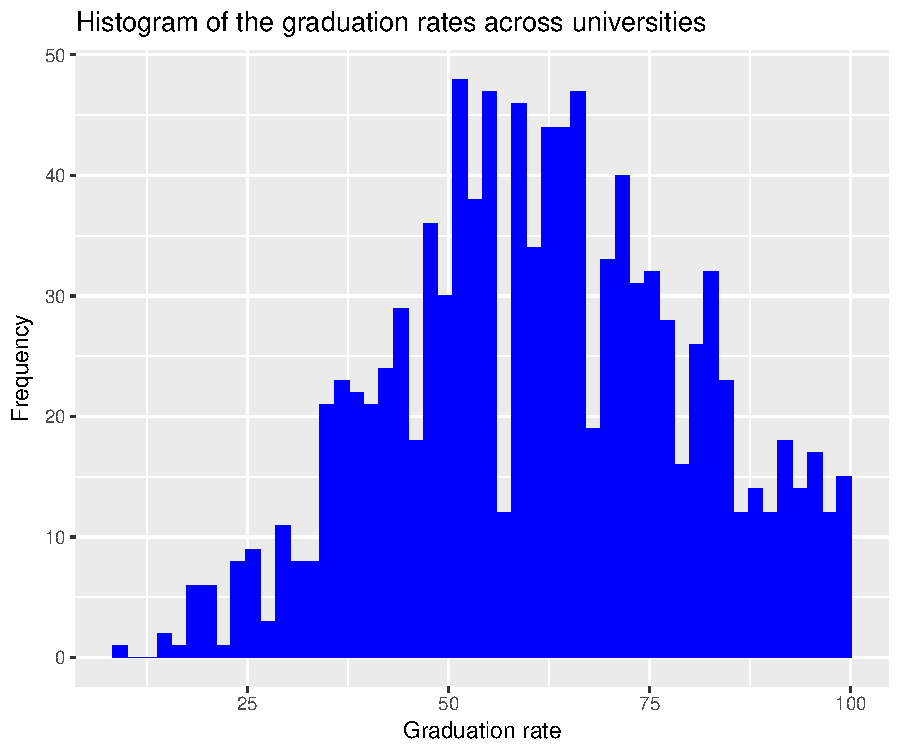
\includegraphics{Midterm_11_01_2016_Answers_files/figure-latex/unnamed-chunk-11-1} \end{flushleft}

\begin{Shaded}
\begin{Highlighting}[]
\CommentTok{# OR hist(college_data$Grad.rate, breaks = 10)}

\CommentTok{# OR college_data %>% ggplot(aes(Grad.rate)) + geom_histogram(bins = 90) +}
\CommentTok{# xlab('Graduation Rate') + ylab('Count') + ggtitle('Graduation Rate}
\CommentTok{# Histogram') + theme_bw()}
\end{Highlighting}
\end{Shaded}

\textbf{Assume all linear model assumptions are met in the following
analyses.}

\section{Question 2: School Type and State vs Graduation
Rate}\label{question-2-school-type-and-state-vs-graduation-rate}

\textbf{a)} Make side to side boxplots of \textbf{graduation rate} vs
\textbf{school type}. Does one type seems to have higher a graduation
rate compared to the other? Write a short summary (max 3 sentences) of
this finding. Does that agree with your intuition about private schools
(\texttt{Schooltype\ =\ 2}) vs.~public schools
(\texttt{Schooltype\ =\ 1})?

\begin{Shaded}
\begin{Highlighting}[]
\CommentTok{# names(college_data)}
\NormalTok{college_data }\OperatorTok\StringTok{ }\KeywordTok{ggplot}\NormalTok{(}\KeywordTok{aes}\NormalTok{(}\DataTypeTok{x =}\NormalTok{ Schooltype, }\DataTypeTok{y =}\NormalTok{ Grad.rate)) }\OperatorTok{+}\StringTok{ }\KeywordTok{geom_boxplot}\NormalTok{() }\OperatorTok{+}\StringTok{ }
\StringTok{    }\KeywordTok{theme}\NormalTok{(}\DataTypeTok{axis.text.x =} \KeywordTok{element_text}\NormalTok{(}\DataTypeTok{angle =} \DecValTok{30}\NormalTok{, }\DataTypeTok{hjust =} \DecValTok{1}\NormalTok{)) }\OperatorTok{+}\StringTok{ }\KeywordTok{labs}\NormalTok{(}\DataTypeTok{title =} \StringTok{"Boxplots of school type versus graduation rate"}\NormalTok{, }
    \DataTypeTok{x =} \StringTok{"School type (1-public, 2-private)"}\NormalTok{, }\DataTypeTok{y =} \StringTok{"graduation rate"}\NormalTok{)}
\end{Highlighting}
\end{Shaded}

\begin{flushleft}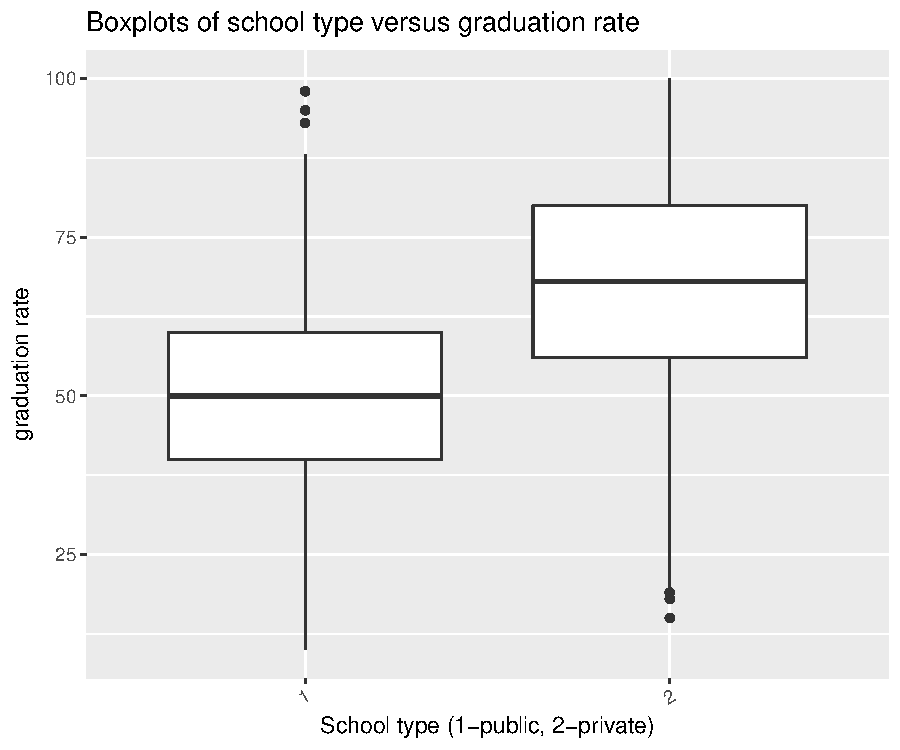
\includegraphics{Midterm_11_01_2016_Answers_files/figure-latex/unnamed-chunk-12-1} \end{flushleft}

\begin{Shaded}
\begin{Highlighting}[]
\CommentTok{# OR boxplot(college_data$Grad.rate ~ college_data$Schooltype)}
\end{Highlighting}
\end{Shaded}

Public schools on left, private schools on right. Private schools appear
to have higher graduation rates.

\textbf{b)} \texttt{fit1}: \texttt{Grad.rate} vs. \texttt{Schooltype}

Perform a test to determine if the mean \texttt{Grad.rate} between the
two school types is different at 0.01 level. Which type has a higher
\texttt{Grad.rate}? Produce a 95\% confidence interval for the mean
difference.

We can perform a t-test:

\begin{Shaded}
\begin{Highlighting}[]
\CommentTok{# ISOLATING JUST PRIVATE SCHOOLS}
\NormalTok{private_grad_rates <-}\StringTok{ }\NormalTok{college_data }\OperatorTok\StringTok{ }\KeywordTok{filter}\NormalTok{(Schooltype }\OperatorTok{==}\StringTok{ }\DecValTok{2}\NormalTok{) }\OperatorTok\StringTok{ }\KeywordTok{select}\NormalTok{(Grad.rate) }\OperatorTok\StringTok{ }
\StringTok{    }\NormalTok{unlist}
\CommentTok{# ISOLATING JUST PUBLIC SCHOOLS}
\NormalTok{public_grad_rates <-}\StringTok{ }\NormalTok{college_data }\OperatorTok\StringTok{ }\KeywordTok{filter}\NormalTok{(Schooltype }\OperatorTok{==}\StringTok{ }\DecValTok{1}\NormalTok{) }\OperatorTok\StringTok{ }\KeywordTok{select}\NormalTok{(Grad.rate) }\OperatorTok\StringTok{ }
\StringTok{    }\NormalTok{unlist}
\KeywordTok{t.test}\NormalTok{(public_grad_rates, private_grad_rates)}
\end{Highlighting}
\end{Shaded}

\begin{verbatim}
## 
##  Welch Two Sample t-test
## 
## data:  public_grad_rates and private_grad_rates
## t = -15.969, df = 788.87, p-value < 2.2e-16
## alternative hypothesis: true difference in means is not equal to 0
## 95 percent confidence interval:
##  -18.88787 -14.75274
## sample estimates:
## mean of x mean of y 
##  50.62108  67.44139
\end{verbatim}

Clarify t-test assumption of normality - looks fine.

\begin{Shaded}
\begin{Highlighting}[]
\KeywordTok{par}\NormalTok{(}\DataTypeTok{mfrow =} \KeywordTok{c}\NormalTok{(}\DecValTok{1}\NormalTok{, }\DecValTok{2}\NormalTok{))}
\KeywordTok{hist}\NormalTok{(private_grad_rates)}
\KeywordTok{hist}\NormalTok{(public_grad_rates)}
\end{Highlighting}
\end{Shaded}

\begin{flushleft}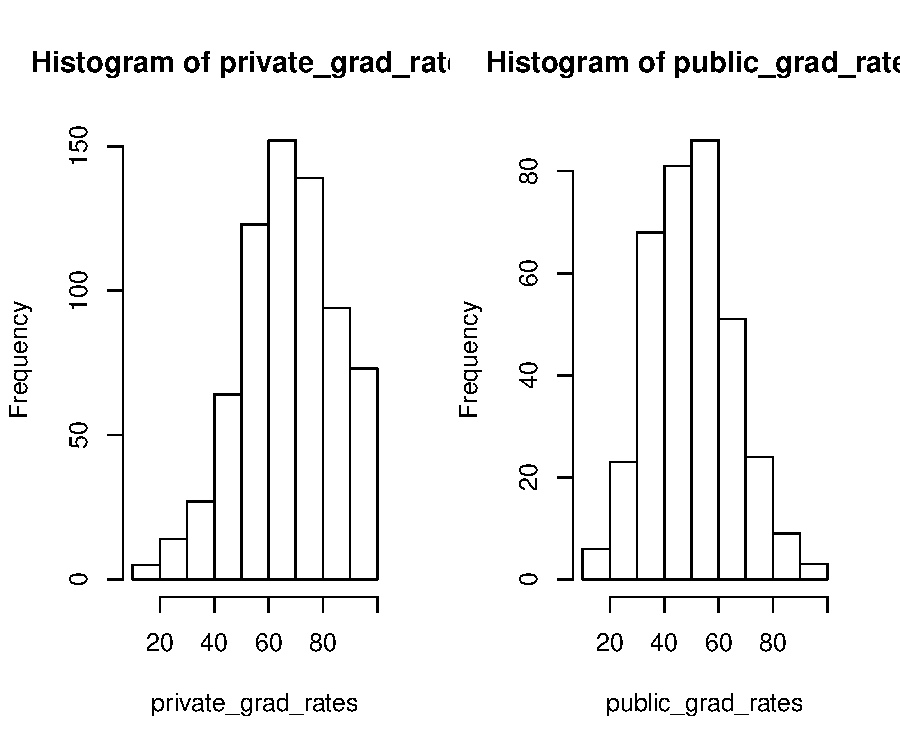
\includegraphics{Midterm_11_01_2016_Answers_files/figure-latex/unnamed-chunk-14-1} \end{flushleft}

Then, we can back out the confidence interval via the above summary
output:

\begin{verbatim}
95 percent confidence interval:
 -18.88787 -14.75274
\end{verbatim}

You can also do a regression based approach, this is probably the easier
one. Note that the results are the same!

\begin{Shaded}
\begin{Highlighting}[]
\NormalTok{fit1 <-}\StringTok{ }\KeywordTok{lm}\NormalTok{(Grad.rate }\OperatorTok{~}\StringTok{ }\NormalTok{Schooltype, }\DataTypeTok{data =}\NormalTok{ college_data)}
\KeywordTok{confint}\NormalTok{(fit1, }\DataTypeTok{parm =} \DecValTok{2}\NormalTok{)}
\end{Highlighting}
\end{Shaded}

\begin{verbatim}
##                2.5 %   97.5 %
## Schooltype2 14.66475 18.97587
\end{verbatim}

\textbf{c)} \texttt{fit1.1}: \texttt{Grad.rate} vs. \texttt{State}

Can we prove that the mean graduation rates are different, at the 0.01
level, among all the states? Which state appears to have the highest
graduation rate, and which state appears to have the lowest graduation
rate? Note that according to standard R-coding \texttt{AK}/Alaska is the
base case in this analysis.

\textbf{Some states have high p-values, that is, they are not
significantly different from Alaska, the base case.}

\begin{Shaded}
\begin{Highlighting}[]
\NormalTok{fit1.}\DecValTok{1}\NormalTok{ <-}\StringTok{ }\KeywordTok{lm}\NormalTok{(Grad.rate }\OperatorTok{~}\StringTok{ }\NormalTok{State, }\DataTypeTok{data =}\NormalTok{ college_data)}
\KeywordTok{summary}\NormalTok{(fit1.}\DecValTok{1}\NormalTok{)}
\end{Highlighting}
\end{Shaded}

\begin{verbatim}
## 
## Call:
## lm(formula = Grad.rate ~ State, data = college_data)
## 
## Residuals:
##     Min      1Q  Median      3Q     Max 
## -47.214 -11.261  -0.238  11.649  44.739 
## 
## Coefficients:
##             Estimate Std. Error t value Pr(>|t|)    
## (Intercept)    15.00      16.76   0.895 0.371091    
## StateAL        33.89      17.22   1.968 0.049375 *  
## StateAR        35.88      17.78   2.018 0.043886 *  
## StateAZ        39.75      18.74   2.121 0.034172 *  
## StateCA        47.07      16.90   2.784 0.005465 ** 
## StateCO        37.08      17.45   2.125 0.033796 *  
## StateCT        59.06      17.28   3.418 0.000656 ***
## StateDC        60.50      18.11   3.341 0.000865 ***
## StateDE        50.00      19.36   2.583 0.009932 ** 
## StateFL        42.13      17.11   2.462 0.013977 *  
## StateGA        36.81      17.02   2.163 0.030814 *  
## StateHI        27.50      20.53   1.339 0.180717    
## StateIA        49.50      17.11   2.893 0.003896 ** 
## StateID        28.33      18.11   1.565 0.117933    
## StateIL        50.21      16.96   2.961 0.003144 ** 
## StateIN        49.44      17.02   2.904 0.003764 ** 
## StateKS        36.93      17.31   2.133 0.033143 *  
## StateKY        43.13      17.31   2.491 0.012885 *  
## StateLA        25.94      17.28   1.501 0.133641    
## StateMA        58.88      16.94   3.476 0.000531 ***
## StateMD        46.05      17.16   2.684 0.007399 ** 
## StateME        54.18      17.51   3.095 0.002026 ** 
## StateMI        44.12      17.08   2.583 0.009950 ** 
## StateMN        53.37      17.20   3.103 0.001969 ** 
## StateMO        43.58      17.11   2.547 0.011001 *  
## StateMS        35.50      17.58   2.019 0.043732 *  
## StateMT        37.29      17.92   2.081 0.037722 *  
## StateNC        41.98      16.96   2.476 0.013470 *  
## StateND        33.33      18.11   1.841 0.065917 .  
## StateNE        44.44      17.67   2.515 0.012050 *  
## StateNH        55.55      17.51   3.173 0.001558 ** 
## StateNJ        45.28      17.09   2.649 0.008207 ** 
## StateNM        28.00      17.78   1.575 0.115613    
## StateNV        26.50      20.53   1.291 0.197079    
## StateNY        51.42      16.86   3.049 0.002355 ** 
## StateOH        54.49      16.97   3.212 0.001363 ** 
## StateOK        27.62      17.40   1.587 0.112720    
## StateOR        39.85      17.40   2.291 0.022196 *  
## StatePA        59.35      16.87   3.518 0.000455 ***
## StateRI        61.63      17.78   3.466 0.000551 ***
## StateSC        47.95      17.18   2.792 0.005346 ** 
## StateSD        38.83      18.11   2.145 0.032212 *  
## StateTN        40.36      17.09   2.361 0.018421 *  
## StateTX        35.26      16.94   2.081 0.037688 *  
## StateUT        22.50      20.53   1.096 0.273367    
## StateVA        50.89      17.00   2.993 0.002829 ** 
## StateVT        58.67      17.45   3.363 0.000802 ***
## StateWA        50.00      17.35   2.882 0.004041 ** 
## StateWI        47.56      17.09   2.782 0.005503 ** 
## StateWV        46.20      17.31   2.669 0.007742 ** 
## StateWY        30.00      23.71   1.265 0.205992    
## ---
## Signif. codes:  0 '***' 0.001 '**' 0.01 '*' 0.05 '.' 0.1 ' ' 1
## 
## Residual standard error: 16.76 on 991 degrees of freedom
## Multiple R-squared:  0.2221, Adjusted R-squared:  0.1829 
## F-statistic: 5.659 on 50 and 991 DF,  p-value: < 2.2e-16
\end{verbatim}

\begin{Shaded}
\begin{Highlighting}[]
\KeywordTok{Anova}\NormalTok{(fit1.}\DecValTok{1}\NormalTok{)}
\end{Highlighting}
\end{Shaded}

\begin{verbatim}
## Anova Table (Type II tests)
## 
## Response: Grad.rate
##           Sum Sq  Df F value    Pr(>F)    
## State      79513  50  5.6595 < 2.2e-16 ***
## Residuals 278462 991                      
## ---
## Signif. codes:  0 '***' 0.001 '**' 0.01 '*' 0.05 '.' 0.1 ' ' 1
\end{verbatim}

\begin{Shaded}
\begin{Highlighting}[]
\CommentTok{# SORT BY P-VALUE IN DESCENDING ORDER}
\KeywordTok{summary}\NormalTok{(fit1.}\DecValTok{1}\NormalTok{) }\OperatorTok\StringTok{ }\NormalTok{broom}\OperatorTok{::}\KeywordTok{tidy}\NormalTok{() }\OperatorTok\StringTok{ }\KeywordTok{arrange}\NormalTok{(}\OperatorTok{-}\NormalTok{p.value) }\OperatorTok\StringTok{ }\NormalTok{head  }\CommentTok{# - p-value makes it descending}
\end{Highlighting}
\end{Shaded}

\begin{verbatim}
##          term estimate std.error statistic   p.value
## 1 (Intercept)  15.0000  16.76279 0.8948389 0.3710905
## 2     StateUT  22.5000  20.53015 1.0959493 0.2733672
## 3     StateWY  30.0000  23.70617 1.2654932 0.2059920
## 4     StateNV  26.5000  20.53015 1.2907847 0.1970794
## 5     StateHI  27.5000  20.53015 1.3394936 0.1807171
## 6     StateLA  25.9375  17.27869 1.5011262 0.1336414
\end{verbatim}

Lowest grad rate states:

\begin{Shaded}
\begin{Highlighting}[]
\CommentTok{# data striated by state, then mean grad rate (ascending order)}
\NormalTok{college_data }\OperatorTok\StringTok{ }\KeywordTok{group_by}\NormalTok{(State) }\OperatorTok\StringTok{ }\KeywordTok{summarize}\NormalTok{(}\DataTypeTok{grad_rate =} \KeywordTok{mean}\NormalTok{(Grad.rate)) }\OperatorTok\StringTok{ }
\StringTok{    }\KeywordTok{arrange}\NormalTok{(grad_rate)}
\end{Highlighting}
\end{Shaded}

\begin{verbatim}
## # A tibble: 51 x 2
##     State grad_rate
##    <fctr>     <dbl>
##  1     AK  15.00000
##  2     UT  37.50000
##  3     LA  40.93750
##  4     NV  41.50000
##  5     HI  42.50000
##  6     OK  42.61538
##  7     NM  43.00000
##  8     ID  43.33333
##  9     WY  45.00000
## 10     ND  48.33333
## # ... with 41 more rows
\end{verbatim}

Highest grad rate states:

\begin{Shaded}
\begin{Highlighting}[]
\CommentTok{# striate by state, then mean grad rate (in descending order)}
\NormalTok{college_data }\OperatorTok\StringTok{ }\KeywordTok{group_by}\NormalTok{(State) }\OperatorTok\StringTok{ }\KeywordTok{summarize}\NormalTok{(}\DataTypeTok{grad_rate =} \KeywordTok{mean}\NormalTok{(Grad.rate)) }\OperatorTok\StringTok{ }
\StringTok{    }\KeywordTok{arrange}\NormalTok{(}\OperatorTok{-}\NormalTok{grad_rate)}
\end{Highlighting}
\end{Shaded}

\begin{verbatim}
## # A tibble: 51 x 2
##     State grad_rate
##    <fctr>     <dbl>
##  1     RI  76.62500
##  2     DC  75.50000
##  3     PA  74.35065
##  4     CT  74.06250
##  5     MA  73.87500
##  6     VT  73.66667
##  7     NH  70.54545
##  8     OH  69.48780
##  9     ME  69.18182
## 10     MN  68.36842
## # ... with 41 more rows
\end{verbatim}

\textbf{d)} \texttt{fit1.2}: \texttt{Grad.rate} vs. \texttt{Schooltype}
and \texttt{State}

Controlling the school type, is the state where the school locates a
useful factor at the .01 level?

\begin{Shaded}
\begin{Highlighting}[]
\NormalTok{fit1.}\DecValTok{2}\NormalTok{ <-}\StringTok{ }\KeywordTok{lm}\NormalTok{(Grad.rate }\OperatorTok{~}\StringTok{ }\NormalTok{Schooltype }\OperatorTok{+}\StringTok{ }\NormalTok{State, }\DataTypeTok{data =}\NormalTok{ college_data)}
\KeywordTok{summary}\NormalTok{(fit1.}\DecValTok{2}\NormalTok{)}
\end{Highlighting}
\end{Shaded}

\begin{verbatim}
## 
## Call:
## lm(formula = Grad.rate ~ Schooltype + State, data = college_data)
## 
## Residuals:
##     Min      1Q  Median      3Q     Max 
## -49.134  -9.722   0.016   9.897  44.135 
## 
## Coefficients:
##             Estimate Std. Error t value Pr(>|t|)    
## (Intercept)   0.8713    15.4929   0.056 0.955161    
## Schooltype2  14.1287     1.0661  13.252  < 2e-16 ***
## StateAL      42.5231    15.8931   2.676 0.007583 ** 
## StateAR      42.9393    16.4025   2.618 0.008983 ** 
## StateAZ      50.3465    17.2991   2.910 0.003691 ** 
## StateCA      51.8572    15.5908   3.326 0.000913 ***
## StateCO      47.6798    16.1072   2.960 0.003148 ** 
## StateCT      62.5947    15.9341   3.928 9.15e-05 ***
## StateDC      60.5000    16.6946   3.624 0.000305 ***
## StateDE      50.0000    17.8473   2.802 0.005185 ** 
## StateFL      46.8346    15.7789   2.968 0.003068 ** 
## StateGA      42.9938    15.7028   2.738 0.006293 ** 
## StateHI      41.6287    18.9599   2.196 0.028351 *  
## StateIA      50.6774    15.7752   3.212 0.001358 ** 
## StateID      37.7524    16.7097   2.259 0.024081 *  
## StateIL      53.2419    15.6408   3.404 0.000691 ***
## StateIN      52.9697    15.6981   3.374 0.000769 ***
## StateKS      40.7010    15.9656   2.549 0.010944 *  
## StateKY      48.7848    15.9688   3.055 0.002311 ** 
## StateLA      35.6510    15.9488   2.235 0.025617 *  
## StateMA      61.5241    15.6177   3.939 8.74e-05 ***
## StateMD      52.1028    15.8265   3.292 0.001030 ** 
## StateME      58.0351    16.1461   3.594 0.000341 ***
## StateMI      50.0929    15.7571   3.179 0.001523 ** 
## StateMN      57.8301    15.8613   3.646 0.000280 ***
## StateMO      47.7042    15.7780   3.023 0.002563 ** 
## StateMS      42.5643    16.2194   2.624 0.008817 ** 
## StateMT      47.3776    16.5409   2.864 0.004268 ** 
## StateNC      46.5768    15.6388   2.978 0.002969 ** 
## StateND      42.7524    16.7097   2.559 0.010659 *  
## StateNE      52.2937    16.3030   3.208 0.001381 ** 
## StateNH      58.1143    16.1447   3.600 0.000335 ***
## StateNJ      52.0618    15.7706   3.301 0.000997 ***
## StateNM      36.8304    16.4073   2.245 0.025004 *  
## StateNV      33.5643    18.9374   1.772 0.076639 .  
## StateNY      55.2852    15.5507   3.555 0.000396 ***
## StateOH      57.5892    15.6453   3.681 0.000245 ***
## StateOK      34.1363    16.0472   2.127 0.033647 *  
## StateOR      43.1066    16.0416   2.687 0.007327 ** 
## StatePA      62.1030    15.5576   3.992 7.04e-05 ***
## StateRI      65.1572    16.3960   3.974 7.58e-05 ***
## StateSC      55.0143    15.8469   3.472 0.000540 ***
## StateSD      45.8977    16.7031   2.748 0.006108 ** 
## StateTN      44.3160    15.7651   2.811 0.005036 ** 
## StateTX      40.4823    15.6283   2.590 0.009729 ** 
## StateUT      36.6287    18.9599   1.932 0.053657 .  
## StateVA      56.1335    15.6805   3.580 0.000360 ***
## StateVT      62.1988    16.0896   3.866 0.000118 ***
## StateWA      56.0551    16.0052   3.502 0.000482 ***
## StateWI      52.6463    15.7670   3.339 0.000872 ***
## StateWV      50.9096    15.9671   3.188 0.001475 ** 
## StateWY      44.1287    21.8844   2.016 0.044023 *  
## ---
## Signif. codes:  0 '***' 0.001 '**' 0.01 '*' 0.05 '.' 0.1 ' ' 1
## 
## Residual standard error: 15.46 on 990 degrees of freedom
## Multiple R-squared:  0.3393, Adjusted R-squared:  0.3053 
## F-statistic:  9.97 on 51 and 990 DF,  p-value: < 2.2e-16
\end{verbatim}

\begin{Shaded}
\begin{Highlighting}[]
\KeywordTok{Anova}\NormalTok{(fit1.}\DecValTok{2}\NormalTok{)}
\end{Highlighting}
\end{Shaded}

\begin{verbatim}
## Anova Table (Type II tests)
## 
## Response: Grad.rate
##            Sum Sq  Df F value    Pr(>F)    
## Schooltype  41957   1 175.628 < 2.2e-16 ***
## State       55615  50   4.656 < 2.2e-16 ***
## Residuals  236506 990                      
## ---
## Signif. codes:  0 '***' 0.001 '**' 0.01 '*' 0.05 '.' 0.1 ' ' 1
\end{verbatim}

\begin{Shaded}
\begin{Highlighting}[]
\CommentTok{# car::Anova(fit1.2)}
\end{Highlighting}
\end{Shaded}

As shown by the Anova test (type II test), yes, it is very much
significant. Yes, as shown clearly in the Anova output, State is
significant at under the 0.01 level.

\section{Question 3: Faculty Effects}\label{question-3-faculty-effects}

The variable \texttt{Pct.fac.degree} summarizes the percentage of
faculty members who hold higher education degrees.

Construct \texttt{fit2}: \texttt{Grad.rate} vs. \texttt{Pct.fac.degree}

\textbf{a)} Report the summary of your linear model. Is
\texttt{Pct.fac.degree} a significant variable in this model at .05
level? How does \texttt{Pct.fac.degree} affect \texttt{Grad.rate}?

\begin{Shaded}
\begin{Highlighting}[]
\NormalTok{fit2 <-}\StringTok{ }\KeywordTok{lm}\NormalTok{(Grad.rate }\OperatorTok{~}\StringTok{ }\NormalTok{Pct.fac.degree, }\DataTypeTok{data =}\NormalTok{ college_data)}
\KeywordTok{summary}\NormalTok{(fit2)}
\end{Highlighting}
\end{Shaded}

\begin{verbatim}
## 
## Call:
## lm(formula = Grad.rate ~ Pct.fac.degree, data = college_data)
## 
## Residuals:
##    Min     1Q Median     3Q    Max 
## -50.87 -12.00   0.21  12.47  54.68 
## 
## Coefficients:
##                Estimate Std. Error t value Pr(>|t|)    
## (Intercept)    35.05981    2.69889   12.99   <2e-16 ***
## Pct.fac.degree  0.34418    0.03405   10.11   <2e-16 ***
## ---
## Signif. codes:  0 '***' 0.001 '**' 0.01 '*' 0.05 '.' 0.1 ' ' 1
## 
## Residual standard error: 17.7 on 1040 degrees of freedom
## Multiple R-squared:  0.08948,    Adjusted R-squared:  0.08861 
## F-statistic: 102.2 on 1 and 1040 DF,  p-value: < 2.2e-16
\end{verbatim}

\begin{Shaded}
\begin{Highlighting}[]
\KeywordTok{Anova}\NormalTok{(fit2)}
\end{Highlighting}
\end{Shaded}

\begin{verbatim}
## Anova Table (Type II tests)
## 
## Response: Grad.rate
##                Sum Sq   Df F value    Pr(>F)    
## Pct.fac.degree  32032    1  102.21 < 2.2e-16 ***
## Residuals      325944 1040                      
## ---
## Signif. codes:  0 '***' 0.001 '**' 0.01 '*' 0.05 '.' 0.1 ' ' 1
\end{verbatim}

\texttt{Pct.fac.degree} is a significant variable in this model at .05
level. For every percent of faculty members who have a higher degree, it
increases graduation rate by 0.34 percent.

\textbf{b)} Make a scatter plot with \(y\) = \texttt{Grad.rate} and
\(x\) = \texttt{Pct.fac.degree}. Overlay \texttt{fit2} onto the plot.

\begin{Shaded}
\begin{Highlighting}[]
\CommentTok{# fit2}
\KeywordTok{plot}\NormalTok{(college_data}\OperatorTok{$}\NormalTok{Pct.fac.degree, college_data}\OperatorTok{$}\NormalTok{Grad.rate, }\DataTypeTok{pch =} \DecValTok{16}\NormalTok{, }\DataTypeTok{xlab =} \StringTok{"Percent of faculty with higher education degrees"}\NormalTok{, }
    \DataTypeTok{ylab =} \StringTok{"Percent graduation rate"}\NormalTok{, }\DataTypeTok{main =} \StringTok{"Universities' graduation rates vs. percent of faculty with higher education degrees"}\NormalTok{)}
\KeywordTok{abline}\NormalTok{(fit2, }\DataTypeTok{col =} \StringTok{"red"}\NormalTok{, }\DataTypeTok{lwd =} \DecValTok{4}\NormalTok{)}
\KeywordTok{abline}\NormalTok{(}\DataTypeTok{h =} \KeywordTok{mean}\NormalTok{(college_data}\OperatorTok{$}\NormalTok{Grad.rate), }\DataTypeTok{lwd =} \DecValTok{5}\NormalTok{, }\DataTypeTok{col =} \StringTok{"blue"}\NormalTok{)}
\end{Highlighting}
\end{Shaded}

\begin{flushleft}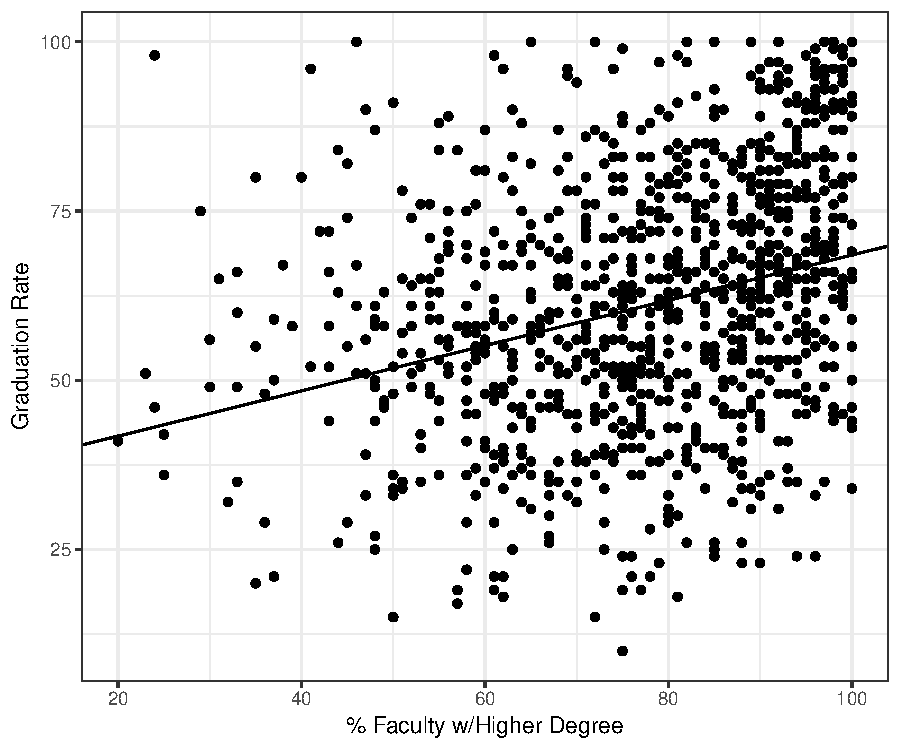
\includegraphics{Midterm_11_01_2016_Answers_files/figure-latex/unnamed-chunk-21-1} \end{flushleft}

\begin{Shaded}
\begin{Highlighting}[]
\CommentTok{# OR college_data %>% ggplot(aes(x = Pct.fac.degree, y= Grad.rate)) +}
\CommentTok{# geom_point() + geom_abline(slope = 0.334418, intercept = 35.05981) +}
\CommentTok{# xlab('% Faculty w/Higher Degree') + ylab('Graduation Rate') + theme_bw()}
\end{Highlighting}
\end{Shaded}

\vspace{.1in}

Construct \texttt{fit2.1}: \texttt{Grad.rate} vs.
\texttt{Pct.fac.degree\ +\ All.test.std}

\begin{Shaded}
\begin{Highlighting}[]
\NormalTok{fit2.}\DecValTok{1}\NormalTok{ <-}\StringTok{ }\KeywordTok{lm}\NormalTok{(Grad.rate }\OperatorTok{~}\StringTok{ }\NormalTok{Pct.fac.degree }\OperatorTok{+}\StringTok{ }\NormalTok{All.test.std, }\DataTypeTok{data =}\NormalTok{ college_data)}
\KeywordTok{summary}\NormalTok{(fit2.}\DecValTok{1}\NormalTok{)}
\end{Highlighting}
\end{Shaded}

\begin{verbatim}
## 
## Call:
## lm(formula = Grad.rate ~ Pct.fac.degree + All.test.std, data = college_data)
## 
## Residuals:
##     Min      1Q  Median      3Q     Max 
## -44.016  -9.744  -0.452   9.181  46.204 
## 
## Coefficients:
##                Estimate Std. Error t value Pr(>|t|)    
## (Intercept)    68.74170    2.69286  25.527   <2e-16 ***
## Pct.fac.degree -0.08538    0.03409  -2.505   0.0124 *  
## All.test.std   12.29484    0.55413  22.188   <2e-16 ***
## ---
## Signif. codes:  0 '***' 0.001 '**' 0.01 '*' 0.05 '.' 0.1 ' ' 1
## 
## Residual standard error: 14.59 on 1039 degrees of freedom
## Multiple R-squared:  0.3822, Adjusted R-squared:  0.381 
## F-statistic: 321.4 on 2 and 1039 DF,  p-value: < 2.2e-16
\end{verbatim}

\begin{Shaded}
\begin{Highlighting}[]
\KeywordTok{Anova}\NormalTok{(fit2.}\DecValTok{1}\NormalTok{)}
\end{Highlighting}
\end{Shaded}

\begin{verbatim}
## Anova Table (Type II tests)
## 
## Response: Grad.rate
##                Sum Sq   Df  F value  Pr(>F)    
## Pct.fac.degree   1335    1   6.2729 0.01241 *  
## All.test.std   104787    1 492.2913 < 2e-16 ***
## Residuals      221157 1039                     
## ---
## Signif. codes:  0 '***' 0.001 '**' 0.01 '*' 0.05 '.' 0.1 ' ' 1
\end{verbatim}

\textbf{c)} Is \texttt{Pct.fac.degree} still a significant variable in
this model at the .05 level?

Yes \textbf{d)} Interpret the coefficent of \texttt{Pct.fac.degree} in
\texttt{fit2.1}. D). All else being held equal, a 1\% increase in
percent of faculty with higher education degrees at a university
corresponds with a .08\% \emph{decrease} in graduation rate.

\emph{This model suggests that it's worse for higher \% of faculty
members to have higher education degrees. }

\begin{Shaded}
\begin{Highlighting}[]
\KeywordTok{summary}\NormalTok{(fit2.}\DecValTok{1}\NormalTok{)}
\end{Highlighting}
\end{Shaded}

\begin{verbatim}
## 
## Call:
## lm(formula = Grad.rate ~ Pct.fac.degree + All.test.std, data = college_data)
## 
## Residuals:
##     Min      1Q  Median      3Q     Max 
## -44.016  -9.744  -0.452   9.181  46.204 
## 
## Coefficients:
##                Estimate Std. Error t value Pr(>|t|)    
## (Intercept)    68.74170    2.69286  25.527   <2e-16 ***
## Pct.fac.degree -0.08538    0.03409  -2.505   0.0124 *  
## All.test.std   12.29484    0.55413  22.188   <2e-16 ***
## ---
## Signif. codes:  0 '***' 0.001 '**' 0.01 '*' 0.05 '.' 0.1 ' ' 1
## 
## Residual standard error: 14.59 on 1039 degrees of freedom
## Multiple R-squared:  0.3822, Adjusted R-squared:  0.381 
## F-statistic: 321.4 on 2 and 1039 DF,  p-value: < 2.2e-16
\end{verbatim}

\textbf{e)} Why might the two estimates of beta for
\texttt{Pct.fac.degree} differ?

\begin{Shaded}
\begin{Highlighting}[]
\CommentTok{# VARIABLES ARE HIGHLY CORRELATED}
\NormalTok{college_data }\OperatorTok\StringTok{ }\KeywordTok{select_if}\NormalTok{(is.numeric) }\OperatorTok\StringTok{ }\KeywordTok{select}\NormalTok{(Pct.fac.degree, All.test.std) }\OperatorTok\StringTok{ }
\StringTok{    }\KeywordTok{ggpairs}\NormalTok{()}
\end{Highlighting}
\end{Shaded}

\begin{flushleft}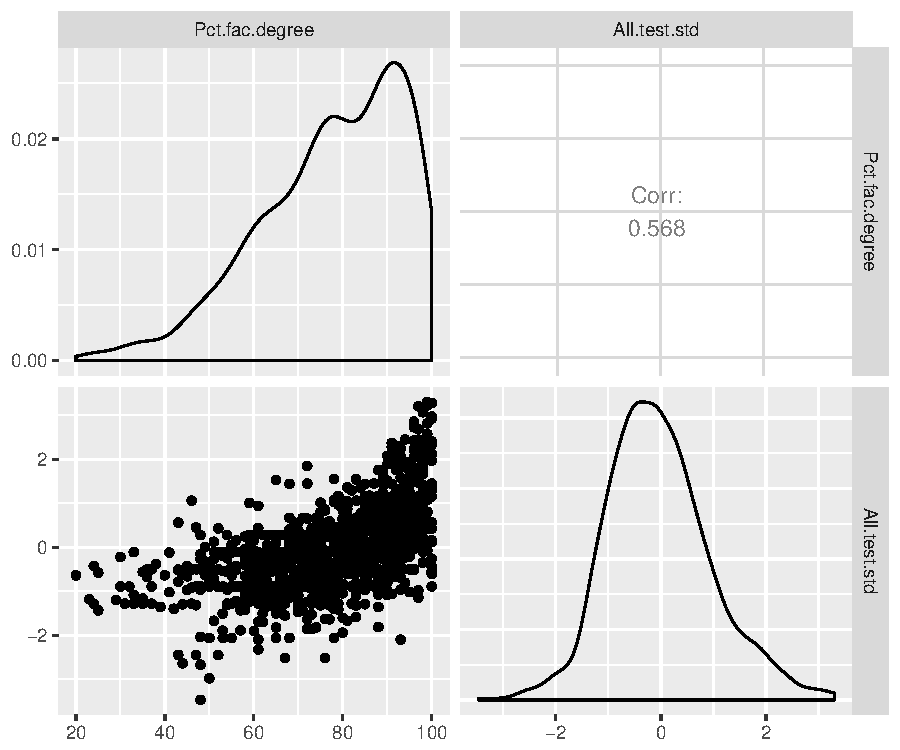
\includegraphics{Midterm_11_01_2016_Answers_files/figure-latex/unnamed-chunk-24-1} \end{flushleft}

\begin{Shaded}
\begin{Highlighting}[]
\NormalTok{college_data }\OperatorTok\StringTok{ }\KeywordTok{select}\NormalTok{(Pct.fac.degree, All.test.std) }\OperatorTok\StringTok{ }\KeywordTok{cor}\NormalTok{()}
\end{Highlighting}
\end{Shaded}

\begin{verbatim}
##                Pct.fac.degree All.test.std
## Pct.fac.degree      1.0000000    0.5679462
## All.test.std        0.5679462    1.0000000
\end{verbatim}

\textbf{This new model controls for the `quality' of students admitted.
The two variables under consideration have a high correlation of
0.5679462, a condition known as collinearity.}

\section{Question 4: Parsimonious Models (all
subsets)}\label{question-4-parsimonious-models-all-subsets}

Construct \texttt{fit3}: a model with all available sensible variables

\begin{Shaded}
\begin{Highlighting}[]
\CommentTok{# FORWARD SELECTION}
\KeywordTok{dim}\NormalTok{(college_data)  }\CommentTok{# n > p}
\end{Highlighting}
\end{Shaded}

\begin{verbatim}
## [1] 1042   13
\end{verbatim}

\begin{Shaded}
\begin{Highlighting}[]
\KeywordTok{names}\NormalTok{(college_data)}
\end{Highlighting}
\end{Shaded}

\begin{verbatim}
##  [1] "Name"            "State"           "Schooltype"     
##  [4] "All.test.std"    "App.accept"      "Acc.Rate"       
##  [7] "Pct.Yield"       "Total.students"  "Student.Faculty"
## [10] "Grad.rate"       "Pct.fac.degree"  "In.Tuition"     
## [13] "Room.board"
\end{verbatim}

\begin{Shaded}
\begin{Highlighting}[]
\NormalTok{college_data2 <-}\StringTok{ }\NormalTok{(college_data)[, }\OperatorTok{-}\DecValTok{1}\NormalTok{]}

\NormalTok{fit3 <-}\StringTok{ }\KeywordTok{regsubsets}\NormalTok{(Grad.rate }\OperatorTok{~}\StringTok{ }\NormalTok{., college_data2, }\DataTypeTok{nvmax =} \DecValTok{12}\NormalTok{, }\DataTypeTok{method =} \StringTok{"forward"}\NormalTok{)}
\KeywordTok{names}\NormalTok{(fit3)}
\end{Highlighting}
\end{Shaded}

\begin{verbatim}
##  [1] "np"        "nrbar"     "d"         "rbar"      "thetab"   
##  [6] "first"     "last"      "vorder"    "tol"       "rss"      
## [11] "bound"     "nvmax"     "ress"      "ir"        "nbest"    
## [16] "lopt"      "il"        "ier"       "xnames"    "method"   
## [21] "force.in"  "force.out" "sserr"     "intercept" "lindep"   
## [26] "nullrss"   "nn"        "call"
\end{verbatim}

\begin{Shaded}
\begin{Highlighting}[]
\KeywordTok{summary}\NormalTok{(fit3)}
\end{Highlighting}
\end{Shaded}

\begin{verbatim}
## Subset selection object
## Call: regsubsets.formula(Grad.rate ~ ., college_data2, nvmax = 12, 
##     method = "forward")
## 60 Variables  (and intercept)
##                 Forced in Forced out
## StateAL             FALSE      FALSE
## StateAR             FALSE      FALSE
## StateAZ             FALSE      FALSE
## StateCA             FALSE      FALSE
## StateCO             FALSE      FALSE
## StateCT             FALSE      FALSE
## StateDC             FALSE      FALSE
## StateDE             FALSE      FALSE
## StateFL             FALSE      FALSE
## StateGA             FALSE      FALSE
## StateHI             FALSE      FALSE
## StateIA             FALSE      FALSE
## StateID             FALSE      FALSE
## StateIL             FALSE      FALSE
## StateIN             FALSE      FALSE
## StateKS             FALSE      FALSE
## StateKY             FALSE      FALSE
## StateLA             FALSE      FALSE
## StateMA             FALSE      FALSE
## StateMD             FALSE      FALSE
## StateME             FALSE      FALSE
## StateMI             FALSE      FALSE
## StateMN             FALSE      FALSE
## StateMO             FALSE      FALSE
## StateMS             FALSE      FALSE
## StateMT             FALSE      FALSE
## StateNC             FALSE      FALSE
## StateND             FALSE      FALSE
## StateNE             FALSE      FALSE
## StateNH             FALSE      FALSE
## StateNJ             FALSE      FALSE
## StateNM             FALSE      FALSE
## StateNV             FALSE      FALSE
## StateNY             FALSE      FALSE
## StateOH             FALSE      FALSE
## StateOK             FALSE      FALSE
## StateOR             FALSE      FALSE
## StatePA             FALSE      FALSE
## StateRI             FALSE      FALSE
## StateSC             FALSE      FALSE
## StateSD             FALSE      FALSE
## StateTN             FALSE      FALSE
## StateTX             FALSE      FALSE
## StateUT             FALSE      FALSE
## StateVA             FALSE      FALSE
## StateVT             FALSE      FALSE
## StateWA             FALSE      FALSE
## StateWI             FALSE      FALSE
## StateWV             FALSE      FALSE
## StateWY             FALSE      FALSE
## Schooltype2         FALSE      FALSE
## All.test.std        FALSE      FALSE
## App.accept          FALSE      FALSE
## Acc.Rate            FALSE      FALSE
## Pct.Yield           FALSE      FALSE
## Total.students      FALSE      FALSE
## Student.Faculty     FALSE      FALSE
## Pct.fac.degree      FALSE      FALSE
## In.Tuition          FALSE      FALSE
## Room.board          FALSE      FALSE
## 1 subsets of each size up to 12
## Selection Algorithm: forward
##           StateAL StateAR StateAZ StateCA StateCO StateCT StateDC StateDE
## 1  ( 1 )  " "     " "     " "     " "     " "     " "     " "     " "    
## 2  ( 1 )  " "     " "     " "     " "     " "     " "     " "     " "    
## 3  ( 1 )  " "     " "     " "     " "     " "     " "     " "     " "    
## 4  ( 1 )  " "     " "     " "     " "     " "     " "     " "     " "    
## 5  ( 1 )  " "     " "     " "     " "     " "     " "     " "     " "    
## 6  ( 1 )  " "     " "     " "     " "     " "     " "     " "     " "    
## 7  ( 1 )  " "     " "     " "     " "     " "     " "     " "     " "    
## 8  ( 1 )  " "     " "     " "     " "     " "     " "     " "     " "    
## 9  ( 1 )  " "     " "     " "     " "     " "     " "     " "     " "    
## 10  ( 1 ) " "     " "     " "     " "     " "     " "     " "     " "    
## 11  ( 1 ) " "     " "     " "     " "     " "     " "     " "     " "    
## 12  ( 1 ) " "     " "     " "     " "     " "     " "     " "     " "    
##           StateFL StateGA StateHI StateIA StateID StateIL StateIN StateKS
## 1  ( 1 )  " "     " "     " "     " "     " "     " "     " "     " "    
## 2  ( 1 )  " "     " "     " "     " "     " "     " "     " "     " "    
## 3  ( 1 )  " "     " "     " "     " "     " "     " "     " "     " "    
## 4  ( 1 )  " "     " "     " "     " "     " "     " "     " "     " "    
## 5  ( 1 )  " "     " "     " "     " "     " "     " "     " "     " "    
## 6  ( 1 )  " "     " "     " "     " "     " "     " "     " "     " "    
## 7  ( 1 )  " "     " "     " "     " "     " "     " "     " "     " "    
## 8  ( 1 )  " "     " "     " "     " "     " "     " "     " "     " "    
## 9  ( 1 )  " "     " "     " "     " "     " "     " "     " "     " "    
## 10  ( 1 ) " "     " "     " "     " "     " "     " "     " "     " "    
## 11  ( 1 ) " "     " "     " "     " "     " "     " "     " "     " "    
## 12  ( 1 ) " "     " "     " "     " "     " "     " "     " "     " "    
##           StateKY StateLA StateMA StateMD StateME StateMI StateMN StateMO
## 1  ( 1 )  " "     " "     " "     " "     " "     " "     " "     " "    
## 2  ( 1 )  " "     " "     " "     " "     " "     " "     " "     " "    
## 3  ( 1 )  " "     " "     " "     " "     " "     " "     " "     " "    
## 4  ( 1 )  " "     "*"     " "     " "     " "     " "     " "     " "    
## 5  ( 1 )  " "     "*"     " "     " "     " "     " "     " "     " "    
## 6  ( 1 )  " "     "*"     " "     " "     " "     " "     " "     " "    
## 7  ( 1 )  " "     "*"     " "     " "     " "     " "     " "     " "    
## 8  ( 1 )  " "     "*"     " "     " "     " "     " "     " "     " "    
## 9  ( 1 )  " "     "*"     "*"     " "     " "     " "     " "     " "    
## 10  ( 1 ) " "     "*"     "*"     " "     " "     " "     " "     " "    
## 11  ( 1 ) " "     "*"     "*"     " "     " "     " "     " "     " "    
## 12  ( 1 ) " "     "*"     "*"     " "     " "     " "     " "     " "    
##           StateMS StateMT StateNC StateND StateNE StateNH StateNJ StateNM
## 1  ( 1 )  " "     " "     " "     " "     " "     " "     " "     " "    
## 2  ( 1 )  " "     " "     " "     " "     " "     " "     " "     " "    
## 3  ( 1 )  " "     " "     " "     " "     " "     " "     " "     " "    
## 4  ( 1 )  " "     " "     " "     " "     " "     " "     " "     " "    
## 5  ( 1 )  " "     " "     " "     " "     " "     " "     " "     " "    
## 6  ( 1 )  " "     " "     " "     " "     " "     " "     " "     " "    
## 7  ( 1 )  " "     " "     " "     " "     " "     " "     " "     " "    
## 8  ( 1 )  " "     " "     " "     " "     " "     " "     " "     " "    
## 9  ( 1 )  " "     " "     " "     " "     " "     " "     " "     " "    
## 10  ( 1 ) " "     " "     " "     " "     " "     " "     " "     " "    
## 11  ( 1 ) " "     " "     " "     " "     " "     " "     " "     " "    
## 12  ( 1 ) " "     " "     " "     " "     " "     " "     " "     " "    
##           StateNV StateNY StateOH StateOK StateOR StatePA StateRI StateSC
## 1  ( 1 )  " "     " "     " "     " "     " "     " "     " "     " "    
## 2  ( 1 )  " "     " "     " "     " "     " "     " "     " "     " "    
## 3  ( 1 )  " "     " "     " "     " "     " "     "*"     " "     " "    
## 4  ( 1 )  " "     " "     " "     " "     " "     "*"     " "     " "    
## 5  ( 1 )  " "     " "     " "     " "     " "     "*"     " "     " "    
## 6  ( 1 )  " "     " "     " "     " "     " "     "*"     " "     " "    
## 7  ( 1 )  " "     " "     " "     "*"     " "     "*"     " "     " "    
## 8  ( 1 )  " "     " "     " "     "*"     " "     "*"     " "     " "    
## 9  ( 1 )  " "     " "     " "     "*"     " "     "*"     " "     " "    
## 10  ( 1 ) " "     " "     " "     "*"     " "     "*"     " "     " "    
## 11  ( 1 ) " "     " "     " "     "*"     "*"     "*"     " "     " "    
## 12  ( 1 ) " "     " "     " "     "*"     "*"     "*"     " "     " "    
##           StateSD StateTN StateTX StateUT StateVA StateVT StateWA StateWI
## 1  ( 1 )  " "     " "     " "     " "     " "     " "     " "     " "    
## 2  ( 1 )  " "     " "     " "     " "     " "     " "     " "     " "    
## 3  ( 1 )  " "     " "     " "     " "     " "     " "     " "     " "    
## 4  ( 1 )  " "     " "     " "     " "     " "     " "     " "     " "    
## 5  ( 1 )  " "     " "     " "     " "     " "     " "     " "     " "    
## 6  ( 1 )  " "     " "     " "     " "     " "     " "     " "     " "    
## 7  ( 1 )  " "     " "     " "     " "     " "     " "     " "     " "    
## 8  ( 1 )  " "     " "     " "     " "     " "     " "     " "     " "    
## 9  ( 1 )  " "     " "     " "     " "     " "     " "     " "     " "    
## 10  ( 1 ) " "     " "     "*"     " "     " "     " "     " "     " "    
## 11  ( 1 ) " "     " "     "*"     " "     " "     " "     " "     " "    
## 12  ( 1 ) " "     " "     "*"     " "     " "     "*"     " "     " "    
##           StateWV StateWY Schooltype2 All.test.std App.accept Acc.Rate
## 1  ( 1 )  " "     " "     " "         "*"          " "        " "     
## 2  ( 1 )  " "     " "     " "         "*"          " "        " "     
## 3  ( 1 )  " "     " "     " "         "*"          " "        " "     
## 4  ( 1 )  " "     " "     " "         "*"          " "        " "     
## 5  ( 1 )  " "     " "     " "         "*"          "*"        " "     
## 6  ( 1 )  " "     " "     " "         "*"          "*"        " "     
## 7  ( 1 )  " "     " "     " "         "*"          "*"        " "     
## 8  ( 1 )  " "     " "     "*"         "*"          "*"        " "     
## 9  ( 1 )  " "     " "     "*"         "*"          "*"        " "     
## 10  ( 1 ) " "     " "     "*"         "*"          "*"        " "     
## 11  ( 1 ) " "     " "     "*"         "*"          "*"        " "     
## 12  ( 1 ) " "     " "     "*"         "*"          "*"        " "     
##           Pct.Yield Total.students Student.Faculty Pct.fac.degree
## 1  ( 1 )  " "       " "            " "             " "           
## 2  ( 1 )  " "       " "            " "             " "           
## 3  ( 1 )  " "       " "            " "             " "           
## 4  ( 1 )  " "       " "            " "             " "           
## 5  ( 1 )  " "       " "            " "             " "           
## 6  ( 1 )  " "       "*"            " "             " "           
## 7  ( 1 )  " "       "*"            " "             " "           
## 8  ( 1 )  " "       "*"            " "             " "           
## 9  ( 1 )  " "       "*"            " "             " "           
## 10  ( 1 ) " "       "*"            " "             " "           
## 11  ( 1 ) " "       "*"            " "             " "           
## 12  ( 1 ) " "       "*"            " "             " "           
##           In.Tuition Room.board
## 1  ( 1 )  " "        " "       
## 2  ( 1 )  "*"        " "       
## 3  ( 1 )  "*"        " "       
## 4  ( 1 )  "*"        " "       
## 5  ( 1 )  "*"        " "       
## 6  ( 1 )  "*"        " "       
## 7  ( 1 )  "*"        " "       
## 8  ( 1 )  "*"        " "       
## 9  ( 1 )  "*"        " "       
## 10  ( 1 ) "*"        " "       
## 11  ( 1 ) "*"        " "       
## 12  ( 1 ) "*"        " "
\end{verbatim}

\begin{Shaded}
\begin{Highlighting}[]
\NormalTok{for.summary <-}\StringTok{ }\KeywordTok{summary}\NormalTok{(fit3)}
\KeywordTok{names}\NormalTok{(for.summary)}
\end{Highlighting}
\end{Shaded}

\begin{verbatim}
## [1] "which"  "rsq"    "rss"    "adjr2"  "cp"     "bic"    "outmat" "obj"
\end{verbatim}

\begin{Shaded}
\begin{Highlighting}[]
\NormalTok{for.summary}\OperatorTok{$}\NormalTok{rsq}
\end{Highlighting}
\end{Shaded}

\begin{verbatim}
##  [1] 0.3784716 0.4864176 0.5011331 0.5066215 0.5122838 0.5267734 0.5317508
##  [8] 0.5361944 0.5406730 0.5444258 0.5482435 0.5515507
\end{verbatim}

\begin{Shaded}
\begin{Highlighting}[]
\CommentTok{# par(mfrow=c(2,2)) plot(for.summary$rss,xlab='Number of Variables',}
\CommentTok{# ylab='RSS',type='l')}
\KeywordTok{plot}\NormalTok{(for.summary}\OperatorTok{$}\NormalTok{adjr2, }\DataTypeTok{xlab =} \StringTok{"Number of Variables"}\NormalTok{, }\DataTypeTok{ylab =} \StringTok{"Adjusted RSq"}\NormalTok{, }
    \DataTypeTok{type =} \StringTok{"l"}\NormalTok{)}
\KeywordTok{which.max}\NormalTok{(for.summary}\OperatorTok{$}\NormalTok{adjr2)}
\end{Highlighting}
\end{Shaded}

\begin{verbatim}
## [1] 12
\end{verbatim}

\begin{Shaded}
\begin{Highlighting}[]
\KeywordTok{points}\NormalTok{(}\KeywordTok{which.max}\NormalTok{(for.summary}\OperatorTok{$}\NormalTok{adjr2), for.summary}\OperatorTok{$}\NormalTok{adjr2[}\KeywordTok{which.max}\NormalTok{(for.summary}\OperatorTok{$}\NormalTok{adjr2)], }
    \DataTypeTok{col =} \StringTok{"red"}\NormalTok{, }\DataTypeTok{cex =} \DecValTok{2}\NormalTok{, }\DataTypeTok{pch =} \DecValTok{20}\NormalTok{)  }\CommentTok{#12 variables}
\end{Highlighting}
\end{Shaded}

\begin{flushleft}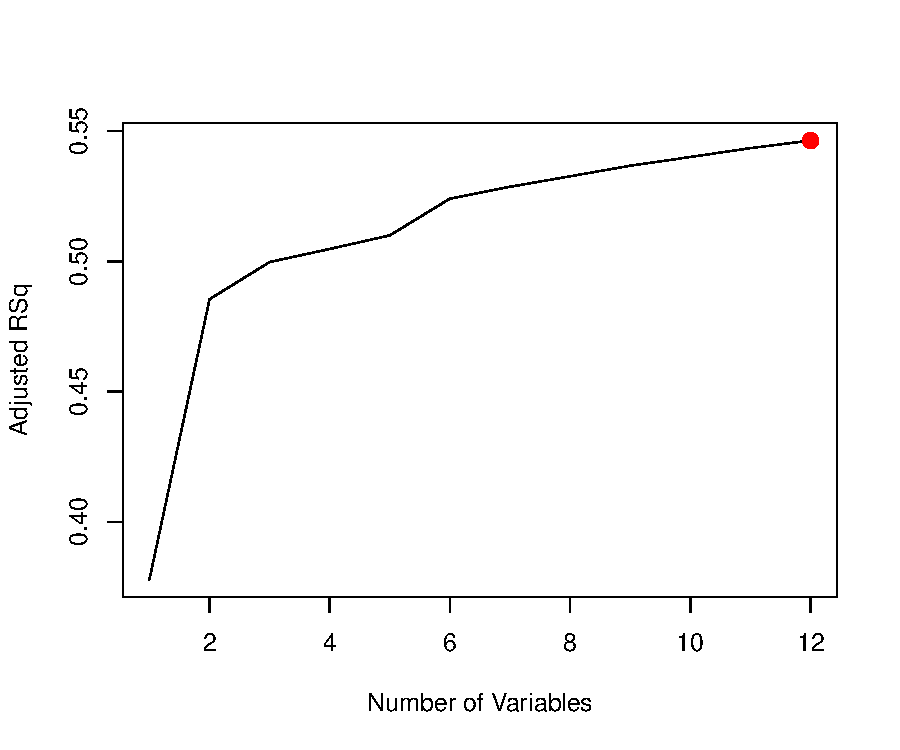
\includegraphics{Midterm_11_01_2016_Answers_files/figure-latex/unnamed-chunk-25-1} \end{flushleft}

\begin{Shaded}
\begin{Highlighting}[]
\KeywordTok{plot}\NormalTok{(for.summary}\OperatorTok{$}\NormalTok{cp, }\DataTypeTok{xlab =} \StringTok{"number of variables"}\NormalTok{, }\DataTypeTok{ylab =} \StringTok{"Cp"}\NormalTok{, }\DataTypeTok{type =} \StringTok{"l"}\NormalTok{)}
\KeywordTok{which.min}\NormalTok{(for.summary}\OperatorTok{$}\NormalTok{cp)}
\end{Highlighting}
\end{Shaded}

\begin{verbatim}
## [1] 12
\end{verbatim}

\begin{Shaded}
\begin{Highlighting}[]
\KeywordTok{points}\NormalTok{(}\KeywordTok{which.min}\NormalTok{(for.summary}\OperatorTok{$}\NormalTok{cp), for.summary}\OperatorTok{$}\NormalTok{cp[}\KeywordTok{which.min}\NormalTok{(for.summary}\OperatorTok{$}\NormalTok{cp)], }
    \DataTypeTok{col =} \StringTok{"red"}\NormalTok{, }\DataTypeTok{cex =} \DecValTok{2}\NormalTok{, }\DataTypeTok{pch =} \DecValTok{20}\NormalTok{)  }\CommentTok{#12 variables}
\end{Highlighting}
\end{Shaded}

\begin{flushleft}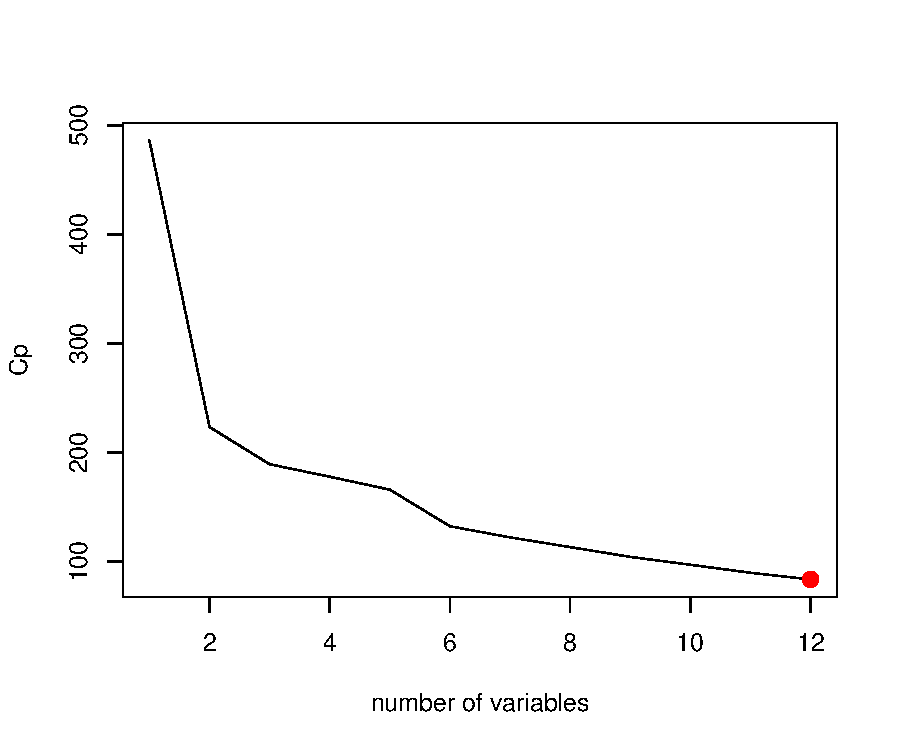
\includegraphics{Midterm_11_01_2016_Answers_files/figure-latex/unnamed-chunk-25-2} \end{flushleft}

\begin{Shaded}
\begin{Highlighting}[]
\KeywordTok{plot}\NormalTok{(for.summary}\OperatorTok{$}\NormalTok{bic, }\DataTypeTok{xlab =} \StringTok{"number of variables"}\NormalTok{, }\DataTypeTok{ylab =} \StringTok{"BIC"}\NormalTok{, }\DataTypeTok{type =} \StringTok{"l"}\NormalTok{)}
\KeywordTok{points}\NormalTok{(}\KeywordTok{which.min}\NormalTok{(for.summary}\OperatorTok{$}\NormalTok{bic), for.summary}\OperatorTok{$}\NormalTok{bic[}\KeywordTok{which.min}\NormalTok{(for.summary}\OperatorTok{$}\NormalTok{bic)], }
    \DataTypeTok{col =} \StringTok{"red"}\NormalTok{, }\DataTypeTok{cex =} \DecValTok{2}\NormalTok{, }\DataTypeTok{pch =} \DecValTok{20}\NormalTok{)  }\CommentTok{# 12 variables}
\end{Highlighting}
\end{Shaded}

\begin{flushleft}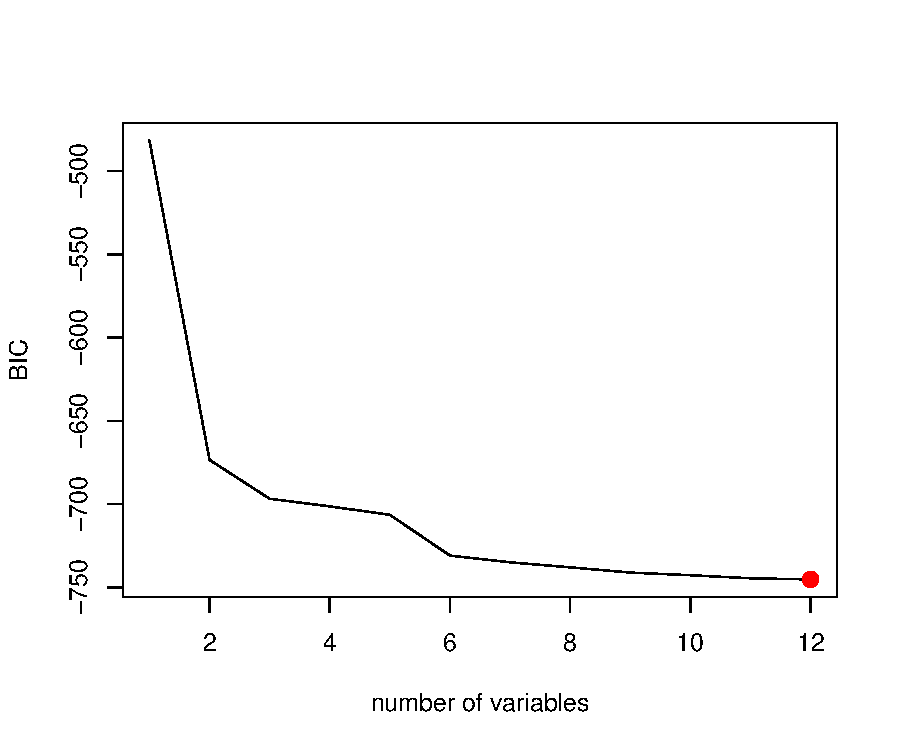
\includegraphics{Midterm_11_01_2016_Answers_files/figure-latex/unnamed-chunk-25-3} \end{flushleft}

\begin{Shaded}
\begin{Highlighting}[]
\CommentTok{# choose to go with 12 variables}
\NormalTok{coef.fit.fwd <-}\StringTok{ }\KeywordTok{coef}\NormalTok{(fit3, }\DecValTok{12}\NormalTok{)}
\NormalTok{var.min <-}\StringTok{ }\KeywordTok{rownames}\NormalTok{(}\KeywordTok{as.matrix}\NormalTok{(coef.fit.fwd))  }\CommentTok{# output the names}
\KeywordTok{print}\NormalTok{(}\StringTok{"============12 variable model using forwards stepwise selection=========="}\NormalTok{)}
\end{Highlighting}
\end{Shaded}

\begin{verbatim}
## [1] "============12 variable model using forwards stepwise selection=========="
\end{verbatim}

\begin{Shaded}
\begin{Highlighting}[]
\NormalTok{lm.input3 <-}\StringTok{ }\KeywordTok{as.formula}\NormalTok{(}\KeywordTok{paste}\NormalTok{(}\StringTok{"violentcrimes.perpop"}\NormalTok{, }\StringTok{"~"}\NormalTok{, }\KeywordTok{paste}\NormalTok{(var.min[}\OperatorTok{-}\DecValTok{1}\NormalTok{], }
    \DataTypeTok{collapse =} \StringTok{"+"}\NormalTok{)))  }\CommentTok{# prepare for lm fomulae}
\NormalTok{lm.input3}
\end{Highlighting}
\end{Shaded}

\begin{verbatim}
## violentcrimes.perpop ~ StateLA + StateMA + StateOK + StateOR + 
##     StatePA + StateTX + StateVT + Schooltype2 + All.test.std + 
##     App.accept + Total.students + In.Tuition
\end{verbatim}

\begin{Shaded}
\begin{Highlighting}[]
\NormalTok{coef.fit.fwd}
\end{Highlighting}
\end{Shaded}

\begin{verbatim}
##    (Intercept)        StateLA        StateMA        StateOK        StateOR 
##   5.215627e+01  -1.041539e+01   6.148881e+00  -1.317666e+01  -1.011695e+01 
##        StatePA        StateTX        StateVT    Schooltype2   All.test.std 
##   8.989426e+00  -5.824833e+00   1.015924e+01   7.151924e+00   8.091627e+00 
##     App.accept Total.students     In.Tuition 
##   2.005926e-03  -6.673084e-04   4.709624e-04
\end{verbatim}

\begin{Shaded}
\begin{Highlighting}[]
\KeywordTok{print}\NormalTok{(}\StringTok{"============BIC & Cp with 4 variables=========="}\NormalTok{)}
\end{Highlighting}
\end{Shaded}

\begin{verbatim}
## [1] "============BIC & Cp with 4 variables=========="
\end{verbatim}

\begin{Shaded}
\begin{Highlighting}[]
\NormalTok{for.summary}\OperatorTok{$}\NormalTok{bic[}\DecValTok{12}\NormalTok{]  }\CommentTok{#-398.7349}
\end{Highlighting}
\end{Shaded}

\begin{verbatim}
## [1] -745.3063
\end{verbatim}

\begin{Shaded}
\begin{Highlighting}[]
\NormalTok{for.summary}\OperatorTok{$}\NormalTok{cp[}\DecValTok{12}\NormalTok{]  }\CommentTok{#9.10198}
\end{Highlighting}
\end{Shaded}

\begin{verbatim}
## [1] 83.67399
\end{verbatim}

There are 1042 entries with 13 variables, which implies that n
\textgreater{} p by some margin. Alsom p is not \emph{too} large,
meaning we could use all subsets, backwards stepwise, or forward
stepwise selection to get the best combination of variables.

\begin{Shaded}
\begin{Highlighting}[]
\NormalTok{fit3 <-}\StringTok{ }\KeywordTok{lm}\NormalTok{(Grad.rate }\OperatorTok{~}\StringTok{ }\NormalTok{. }\OperatorTok{-}\StringTok{ }\NormalTok{Name, }\DataTypeTok{data =}\NormalTok{ college_data)}
\KeywordTok{summary}\NormalTok{(fit3)}
\end{Highlighting}
\end{Shaded}

\begin{verbatim}
## 
## Call:
## lm(formula = Grad.rate ~ . - Name, data = college_data)
## 
## Residuals:
##     Min      1Q  Median      3Q     Max 
## -40.996  -7.286  -0.118   6.484  43.954 
## 
## Coefficients:
##                   Estimate Std. Error t value Pr(>|t|)    
## (Intercept)      1.130e+01  1.296e+01   0.872 0.383560    
## StateAL          3.761e+01  1.245e+01   3.021 0.002581 ** 
## StateAR          3.630e+01  1.287e+01   2.822 0.004876 ** 
## StateAZ          4.242e+01  1.358e+01   3.125 0.001832 ** 
## StateCA          4.131e+01  1.223e+01   3.377 0.000762 ***
## StateCO          3.957e+01  1.262e+01   3.135 0.001768 ** 
## StateCT          5.215e+01  1.250e+01   4.171 3.30e-05 ***
## StateDC          4.636e+01  1.311e+01   3.536 0.000425 ***
## StateDE          4.726e+01  1.401e+01   3.374 0.000769 ***
## StateFL          4.185e+01  1.235e+01   3.388 0.000732 ***
## StateGA          3.873e+01  1.229e+01   3.152 0.001669 ** 
## StateHI          3.842e+01  1.484e+01   2.588 0.009785 ** 
## StateIA          4.490e+01  1.237e+01   3.630 0.000298 ***
## StateID          3.302e+01  1.310e+01   2.520 0.011882 *  
## StateIL          4.596e+01  1.225e+01   3.753 0.000185 ***
## StateIN          4.662e+01  1.230e+01   3.789 0.000160 ***
## StateKS          3.824e+01  1.250e+01   3.058 0.002289 ** 
## StateKY          4.530e+01  1.250e+01   3.625 0.000304 ***
## StateLA          3.472e+01  1.253e+01   2.772 0.005681 ** 
## StateMA          5.088e+01  1.226e+01   4.150 3.62e-05 ***
## StateMD          4.232e+01  1.240e+01   3.413 0.000669 ***
## StateME          5.166e+01  1.267e+01   4.077 4.92e-05 ***
## StateMI          4.220e+01  1.236e+01   3.415 0.000664 ***
## StateMN          4.833e+01  1.244e+01   3.884 0.000110 ***
## StateMO          4.109e+01  1.235e+01   3.327 0.000912 ***
## StateMS          4.264e+01  1.272e+01   3.353 0.000830 ***
## StateMT          4.345e+01  1.298e+01   3.347 0.000848 ***
## StateNC          4.451e+01  1.223e+01   3.638 0.000289 ***
## StateND          3.961e+01  1.313e+01   3.016 0.002627 ** 
## StateNE          4.736e+01  1.279e+01   3.703 0.000225 ***
## StateNH          5.297e+01  1.266e+01   4.183 3.13e-05 ***
## StateNJ          4.247e+01  1.236e+01   3.435 0.000618 ***
## StateNM          3.377e+01  1.285e+01   2.628 0.008717 ** 
## StateNV          3.213e+01  1.484e+01   2.164 0.030693 *  
## StateNY          4.467e+01  1.219e+01   3.665 0.000261 ***
## StateOH          5.017e+01  1.227e+01   4.089 4.69e-05 ***
## StateOK          3.081e+01  1.259e+01   2.447 0.014591 *  
## StateOR          3.530e+01  1.258e+01   2.806 0.005120 ** 
## StatePA          5.380e+01  1.219e+01   4.413 1.13e-05 ***
## StateRI          5.485e+01  1.289e+01   4.254 2.30e-05 ***
## StateSC          5.172e+01  1.241e+01   4.167 3.36e-05 ***
## StateSD          4.470e+01  1.313e+01   3.405 0.000687 ***
## StateTN          3.816e+01  1.234e+01   3.092 0.002045 ** 
## StateTX          3.745e+01  1.224e+01   3.060 0.002274 ** 
## StateUT          3.362e+01  1.491e+01   2.254 0.024393 *  
## StateVA          4.815e+01  1.227e+01   3.923 9.36e-05 ***
## StateVT          5.581e+01  1.264e+01   4.417 1.11e-05 ***
## StateWA          4.806e+01  1.254e+01   3.833 0.000134 ***
## StateWI          4.608e+01  1.236e+01   3.728 0.000204 ***
## StateWV          5.025e+01  1.251e+01   4.017 6.35e-05 ***
## StateWY          3.526e+01  1.715e+01   2.055 0.040100 *  
## Schooltype2      9.407e+00  1.822e+00   5.163 2.95e-07 ***
## All.test.std     8.803e+00  6.428e-01  13.695  < 2e-16 ***
## App.accept       1.697e-03  3.274e-04   5.182 2.67e-07 ***
## Acc.Rate        -5.636e-02  3.130e-02  -1.800 0.072105 .  
## Pct.Yield        1.824e-02  3.476e-02   0.525 0.599853    
## Total.students  -6.187e-04  1.462e-04  -4.231 2.55e-05 ***
## Student.Faculty  3.819e-02  9.333e-02   0.409 0.682495    
## Pct.fac.degree  -1.467e-02  3.413e-02  -0.430 0.667351    
## In.Tuition       3.947e-06  1.971e-04   0.020 0.984030    
## Room.board       7.916e-04  6.016e-04   1.316 0.188541    
## ---
## Signif. codes:  0 '***' 0.001 '**' 0.01 '*' 0.05 '.' 0.1 ' ' 1
## 
## Residual standard error: 12.08 on 981 degrees of freedom
## Multiple R-squared:  0.5999, Adjusted R-squared:  0.5755 
## F-statistic: 24.52 on 60 and 981 DF,  p-value: < 2.2e-16
\end{verbatim}

\begin{Shaded}
\begin{Highlighting}[]
\KeywordTok{Anova}\NormalTok{(fit3)}
\end{Highlighting}
\end{Shaded}

\begin{verbatim}
## Anova Table (Type II tests)
## 
## Response: Grad.rate
##                 Sum Sq  Df  F value    Pr(>F)    
## State            28575  50   3.9148 < 2.2e-16 ***
## Schooltype        3891   1  26.6535 2.946e-07 ***
## All.test.std     27381   1 187.5645 < 2.2e-16 ***
## App.accept        3919   1  26.8483 2.671e-07 ***
## Acc.Rate           473   1   3.2414    0.0721 .  
## Pct.Yield           40   1   0.2754    0.5999    
## Total.students    2613   1  17.8994 2.547e-05 ***
## Student.Faculty     24   1   0.1674    0.6825    
## Pct.fac.degree      27   1   0.1848    0.6674    
## In.Tuition           0   1   0.0004    0.9840    
## Room.board         253   1   1.7314    0.1885    
## Residuals       143209 981                       
## ---
## Signif. codes:  0 '***' 0.001 '**' 0.01 '*' 0.05 '.' 0.1 ' ' 1
\end{verbatim}

Based on fit3, answer the following questions:

\textbf{a)} Is \texttt{State} a significant variable at .01 level after
controlling for all other variables in the model? Provide an appropriate
test.

We can do Anova test - State is significant.

\begin{Shaded}
\begin{Highlighting}[]
\NormalTok{car}\OperatorTok{::}\KeywordTok{Anova}\NormalTok{(fit3)}
\end{Highlighting}
\end{Shaded}

\begin{verbatim}
## Anova Table (Type II tests)
## 
## Response: Grad.rate
##                 Sum Sq  Df  F value    Pr(>F)    
## State            28575  50   3.9148 < 2.2e-16 ***
## Schooltype        3891   1  26.6535 2.946e-07 ***
## All.test.std     27381   1 187.5645 < 2.2e-16 ***
## App.accept        3919   1  26.8483 2.671e-07 ***
## Acc.Rate           473   1   3.2414    0.0721 .  
## Pct.Yield           40   1   0.2754    0.5999    
## Total.students    2613   1  17.8994 2.547e-05 ***
## Student.Faculty     24   1   0.1674    0.6825    
## Pct.fac.degree      27   1   0.1848    0.6674    
## In.Tuition           0   1   0.0004    0.9840    
## Room.board         253   1   1.7314    0.1885    
## Residuals       143209 981                       
## ---
## Signif. codes:  0 '***' 0.001 '**' 0.01 '*' 0.05 '.' 0.1 ' ' 1
\end{verbatim}

\textbf{b)} If you want to kick one variable out from this model such
that the resulting model would have the smallest possible RSS, which
variable would you choose, and why?

Kick out instate tuition - variable with smallest F-value / least
importance. Kick out -- smallest F value or largest P value

\vspace{.1in}

Remove \texttt{State} from the data under consideration but include all
other variables. Construct \texttt{fit4}: a parsimonious model, using
regusubsets with exhaustive search.

\begin{Shaded}
\begin{Highlighting}[]
\NormalTok{fit.exh <-}\StringTok{ }\KeywordTok{regsubsets}\NormalTok{(Grad.rate }\OperatorTok{~}\StringTok{ }\NormalTok{. }\OperatorTok{-}\StringTok{ }\NormalTok{Name }\OperatorTok{-}\StringTok{ }\NormalTok{State, college_data, }\DataTypeTok{nvmax =} \DecValTok{12}\NormalTok{, }
    \DataTypeTok{method =} \StringTok{"exhaustive"}\NormalTok{)}
\NormalTok{exh.summary <-}\StringTok{ }\KeywordTok{summary}\NormalTok{(fit3)}
\CommentTok{# exh.summary plot(exh.summary$adjr2,xlab='Number of Variables',}
\CommentTok{# ylab='Adjusted RSq',type='l') which.max(exh.summary$adjr2)}
\CommentTok{# points(which.max(exh.summary$adjr2),exh.summary$adjr2[which.max(exh.summary$adjr2)],}
\CommentTok{# col='red',cex=2,pch=20) #12 variables plot(exh.summary$cp,xlab='number of}
\CommentTok{# variables',ylab='Cp', type = 'l') which.min(exh.summary$cp)}
\CommentTok{# points(which.min(exh.summary$cp),exh.summary$cp[which.min(exh.summary$cp)],col='red',cex=2,pch=20)}
\CommentTok{# #12 variables plot(exh.summary$bic,xlab='number of variables',ylab='BIC',}
\CommentTok{# type = 'l')}
\CommentTok{# points(which.min(exh.summary$bic),exh.summary$bic[which.min(exh.summary$bic)],col='red',cex=2,pch=20)}
\CommentTok{# # 12 variables}
\end{Highlighting}
\end{Shaded}

\begin{Shaded}
\begin{Highlighting}[]
\NormalTok{colleges_sub <-}\StringTok{ }\NormalTok{college_data }\OperatorTok\StringTok{ }\KeywordTok{select}\NormalTok{(}\OperatorTok{-}\NormalTok{Name, }\OperatorTok{-}\NormalTok{State)}
\NormalTok{x_col <-}\StringTok{ }\KeywordTok{model.matrix}\NormalTok{(Grad.rate }\OperatorTok{~}\StringTok{ }\NormalTok{., colleges_sub)[, }\OperatorTok{-}\DecValTok{1}\NormalTok{]}
\NormalTok{y_col <-}\StringTok{ }\NormalTok{college_data}\OperatorTok{$}\NormalTok{Grad.rate}
\NormalTok{reg_search <-}\StringTok{ }\KeywordTok{regsubsets}\NormalTok{(x_col, y_col, }\DataTypeTok{method =} \StringTok{"exhaustive"}\NormalTok{)}
\KeywordTok{summary}\NormalTok{(reg_search)}
\end{Highlighting}
\end{Shaded}

\begin{verbatim}
## Subset selection object
## 10 Variables  (and intercept)
##                 Forced in Forced out
## Schooltype2         FALSE      FALSE
## All.test.std        FALSE      FALSE
## App.accept          FALSE      FALSE
## Acc.Rate            FALSE      FALSE
## Pct.Yield           FALSE      FALSE
## Total.students      FALSE      FALSE
## Student.Faculty     FALSE      FALSE
## Pct.fac.degree      FALSE      FALSE
## In.Tuition          FALSE      FALSE
## Room.board          FALSE      FALSE
## 1 subsets of each size up to 8
## Selection Algorithm: exhaustive
##          Schooltype2 All.test.std App.accept Acc.Rate Pct.Yield
## 1  ( 1 ) " "         "*"          " "        " "      " "      
## 2  ( 1 ) " "         "*"          " "        " "      " "      
## 3  ( 1 ) " "         "*"          " "        " "      "*"      
## 4  ( 1 ) " "         "*"          "*"        " "      " "      
## 5  ( 1 ) " "         "*"          "*"        "*"      " "      
## 6  ( 1 ) "*"         "*"          "*"        "*"      " "      
## 7  ( 1 ) "*"         "*"          "*"        "*"      " "      
## 8  ( 1 ) "*"         "*"          "*"        "*"      " "      
##          Total.students Student.Faculty Pct.fac.degree In.Tuition
## 1  ( 1 ) " "            " "             " "            " "       
## 2  ( 1 ) " "            " "             " "            "*"       
## 3  ( 1 ) " "            " "             " "            "*"       
## 4  ( 1 ) "*"            " "             " "            "*"       
## 5  ( 1 ) "*"            " "             " "            "*"       
## 6  ( 1 ) "*"            " "             " "            "*"       
## 7  ( 1 ) "*"            " "             " "            "*"       
## 8  ( 1 ) "*"            " "             "*"            "*"       
##          Room.board
## 1  ( 1 ) " "       
## 2  ( 1 ) " "       
## 3  ( 1 ) " "       
## 4  ( 1 ) " "       
## 5  ( 1 ) " "       
## 6  ( 1 ) " "       
## 7  ( 1 ) "*"       
## 8  ( 1 ) "*"
\end{verbatim}

\begin{Shaded}
\begin{Highlighting}[]
\NormalTok{reg.summary <-}\StringTok{ }\KeywordTok{summary}\NormalTok{(reg_search)}
\end{Highlighting}
\end{Shaded}

\textbf{c)} Show the Cp plot and also show the BIC plot. Based on the
two plots, which is the most desirable model size? Why?

\begin{Shaded}
\begin{Highlighting}[]
\KeywordTok{par}\NormalTok{(}\DataTypeTok{mfrow =} \KeywordTok{c}\NormalTok{(}\DecValTok{2}\NormalTok{, }\DecValTok{2}\NormalTok{))}
\CommentTok{# Cp PLOT}
\KeywordTok{names}\NormalTok{(reg.summary)}
\end{Highlighting}
\end{Shaded}

\begin{verbatim}
## [1] "which"  "rsq"    "rss"    "adjr2"  "cp"     "bic"    "outmat" "obj"
\end{verbatim}

\begin{Shaded}
\begin{Highlighting}[]
\KeywordTok{plot}\NormalTok{(reg.summary}\OperatorTok{$}\NormalTok{cp, }\DataTypeTok{xlab =} \StringTok{"number of variables"}\NormalTok{, }\DataTypeTok{ylab =} \StringTok{"Cp"}\NormalTok{, }\DataTypeTok{type =} \StringTok{"l"}\NormalTok{)}
\KeywordTok{points}\NormalTok{(}\KeywordTok{which.min}\NormalTok{(reg.summary}\OperatorTok{$}\NormalTok{cp), reg.summary}\OperatorTok{$}\NormalTok{cp[}\KeywordTok{which.min}\NormalTok{(reg.summary}\OperatorTok{$}\NormalTok{cp)], }
    \DataTypeTok{col =} \StringTok{"red"}\NormalTok{, }\DataTypeTok{cex =} \DecValTok{2}\NormalTok{, }\DataTypeTok{pch =} \DecValTok{20}\NormalTok{)  }\CommentTok{# 7 vars}

\CommentTok{# BIC PLOT}
\KeywordTok{plot}\NormalTok{(reg.summary}\OperatorTok{$}\NormalTok{bic, }\DataTypeTok{xlab =} \StringTok{"number of variables"}\NormalTok{, }\DataTypeTok{ylab =} \StringTok{"BIC"}\NormalTok{, }\DataTypeTok{type =} \StringTok{"l"}\NormalTok{)}
\KeywordTok{which.min}\NormalTok{(reg.summary}\OperatorTok{$}\NormalTok{bic)}
\end{Highlighting}
\end{Shaded}

\begin{verbatim}
## [1] 6
\end{verbatim}

\begin{Shaded}
\begin{Highlighting}[]
\KeywordTok{points}\NormalTok{(}\DecValTok{6}\NormalTok{, reg.summary}\OperatorTok{$}\NormalTok{bic[}\DecValTok{6}\NormalTok{], }\DataTypeTok{col =} \StringTok{"red"}\NormalTok{, }\DataTypeTok{cex =} \DecValTok{2}\NormalTok{, }\DataTypeTok{pch =} \DecValTok{20}\NormalTok{)  }\CommentTok{# 6 vars}
\CommentTok{# OR par(mfrow = c(1, 2)) plot(summary(reg_search)$bic, main = 'BIC Plot')}
\CommentTok{# plot(summary(reg_search)$cp, main = 'CP Plot') # find min via BIC:}
\CommentTok{# which(summary(reg_search)$bic == min(summary(reg_search)$bic)) # find min}
\CommentTok{# via CP: which(summary(reg_search)$cp == min(summary(reg_search)$cp))}
\end{Highlighting}
\end{Shaded}

\begin{flushleft}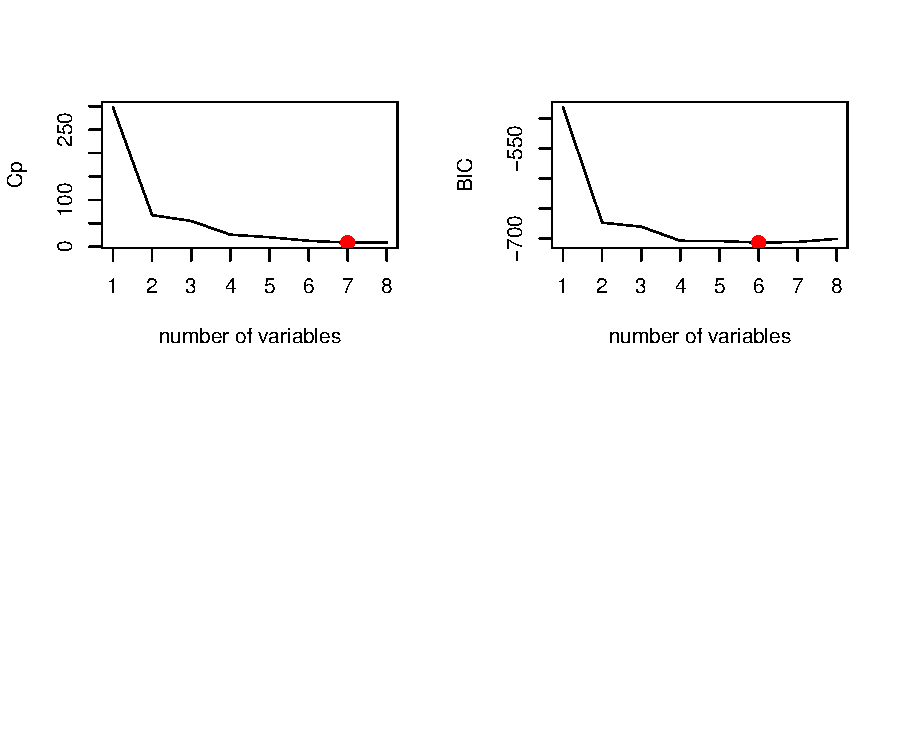
\includegraphics{Midterm_11_01_2016_Answers_files/figure-latex/unnamed-chunk-30-1} \end{flushleft}

\textbf{d)} Regardless of your answer in c), report the 4-variable model
chosen by regsubsets. To save time we will not pursue further.

\begin{Shaded}
\begin{Highlighting}[]
\CommentTok{# model w/ 4 variables}
\NormalTok{coef.exh <-}\StringTok{ }\KeywordTok{coef}\NormalTok{(reg_search, }\DecValTok{4}\NormalTok{)}
\NormalTok{var.min <-}\StringTok{ }\KeywordTok{rownames}\NormalTok{(}\KeywordTok{as.matrix}\NormalTok{(coef.exh))  }\CommentTok{# output the names}
\NormalTok{var.min}
\end{Highlighting}
\end{Shaded}

\begin{verbatim}
## [1] "(Intercept)"    "All.test.std"   "App.accept"     "Total.students"
## [5] "In.Tuition"
\end{verbatim}

\begin{Shaded}
\begin{Highlighting}[]
\KeywordTok{print}\NormalTok{(}\StringTok{"===========4 variable model using all subsets=========="}\NormalTok{)}
\end{Highlighting}
\end{Shaded}

\begin{verbatim}
## [1] "===========4 variable model using all subsets=========="
\end{verbatim}

\begin{Shaded}
\begin{Highlighting}[]
\NormalTok{lm.input2 <-}\StringTok{ }\KeywordTok{as.formula}\NormalTok{(}\KeywordTok{paste}\NormalTok{(}\StringTok{"Grad.rate"}\NormalTok{, }\StringTok{"~"}\NormalTok{, }\KeywordTok{paste}\NormalTok{(var.min[}\OperatorTok{-}\DecValTok{1}\NormalTok{], }\DataTypeTok{collapse =} \StringTok{"+"}\NormalTok{)))}
\NormalTok{lm.input2}
\end{Highlighting}
\end{Shaded}

\begin{verbatim}
## Grad.rate ~ All.test.std + App.accept + Total.students + In.Tuition
\end{verbatim}

\begin{Shaded}
\begin{Highlighting}[]
\NormalTok{coef.exh}
\end{Highlighting}
\end{Shaded}

\begin{verbatim}
##    (Intercept)   All.test.std     App.accept Total.students     In.Tuition 
##  51.4523981254   6.9493748873   0.0021146658  -0.0007963168   0.0012004866
\end{verbatim}

\begin{Shaded}
\begin{Highlighting}[]
\KeywordTok{print}\NormalTok{(}\StringTok{"============BIC & Cp with 4 variables=========="}\NormalTok{)}
\end{Highlighting}
\end{Shaded}

\begin{verbatim}
## [1] "============BIC & Cp with 4 variables=========="
\end{verbatim}

\begin{Shaded}
\begin{Highlighting}[]
\NormalTok{reg.summary}\OperatorTok{$}\NormalTok{bic[}\DecValTok{4}\NormalTok{]  }\CommentTok{# -703.7376}
\end{Highlighting}
\end{Shaded}

\begin{verbatim}
## [1] -703.7376
\end{verbatim}

\begin{Shaded}
\begin{Highlighting}[]
\NormalTok{reg.summary}\OperatorTok{$}\NormalTok{cp[}\DecValTok{4}\NormalTok{]  }\CommentTok{# 25.63655}
\end{Highlighting}
\end{Shaded}

\begin{verbatim}
## [1] 25.63655
\end{verbatim}

``All.test.std'' ``App.accept'' ``Total.students'' ``In.Tuition''
Grad.rate \textasciitilde{} All.test.std + App.accept + Total.students +
In.Tuition
\texttt{All.test.std,\ App.accept,\ Total.students,\ In.tuition}

\section{Question 5: Parsimonious Models
(LASSO)}\label{question-5-parsimonious-models-lasso}

Use LASSO for model selection, again making sure to do so without
including the \texttt{State} variable in the LASSO process.

\textbf{a)} Run \texttt{cv.glmnet()} with \texttt{set.seed(12)}. Plot
\texttt{cmv} vs. \texttt{lambda}.

\begin{Shaded}
\begin{Highlighting}[]
\KeywordTok{set.seed}\NormalTok{(}\DecValTok{12}\NormalTok{)}
\KeywordTok{names}\NormalTok{(college_data)}
\end{Highlighting}
\end{Shaded}

\begin{verbatim}
##  [1] "Name"            "State"           "Schooltype"     
##  [4] "All.test.std"    "App.accept"      "Acc.Rate"       
##  [7] "Pct.Yield"       "Total.students"  "Student.Faculty"
## [10] "Grad.rate"       "Pct.fac.degree"  "In.Tuition"     
## [13] "Room.board"
\end{verbatim}

\begin{Shaded}
\begin{Highlighting}[]
\CommentTok{# extract y, Grad.rate}
\NormalTok{Y <-}\StringTok{ }\NormalTok{college_data}\OperatorTok{$}\NormalTok{Grad.rate}
\NormalTok{X <-}\StringTok{ }\KeywordTok{model.matrix}\NormalTok{(Grad.rate }\OperatorTok{~}\StringTok{ }\NormalTok{. }\OperatorTok{-}\StringTok{ }\NormalTok{Name }\OperatorTok{-}\StringTok{ }\NormalTok{State, }\DataTypeTok{data =}\NormalTok{ college_data)[, }\OperatorTok{-}\DecValTok{1}\NormalTok{]}
\CommentTok{# colnames(X)}
\NormalTok{fit.lasso.cv <-}\StringTok{ }\KeywordTok{cv.glmnet}\NormalTok{(X, Y, }\DataTypeTok{alpha =} \DecValTok{1}\NormalTok{, }\DataTypeTok{nfolds =} \DecValTok{10}\NormalTok{)}
\NormalTok{fit.lasso.cv}\OperatorTok{$}\NormalTok{lambda.1se  }\CommentTok{#1.222679}
\end{Highlighting}
\end{Shaded}

\begin{verbatim}
## [1] 1.222679
\end{verbatim}

\begin{Shaded}
\begin{Highlighting}[]
\KeywordTok{plot}\NormalTok{(fit.lasso.cv)  }\CommentTok{# plots the possible values for lambda}
\end{Highlighting}
\end{Shaded}

\begin{flushleft}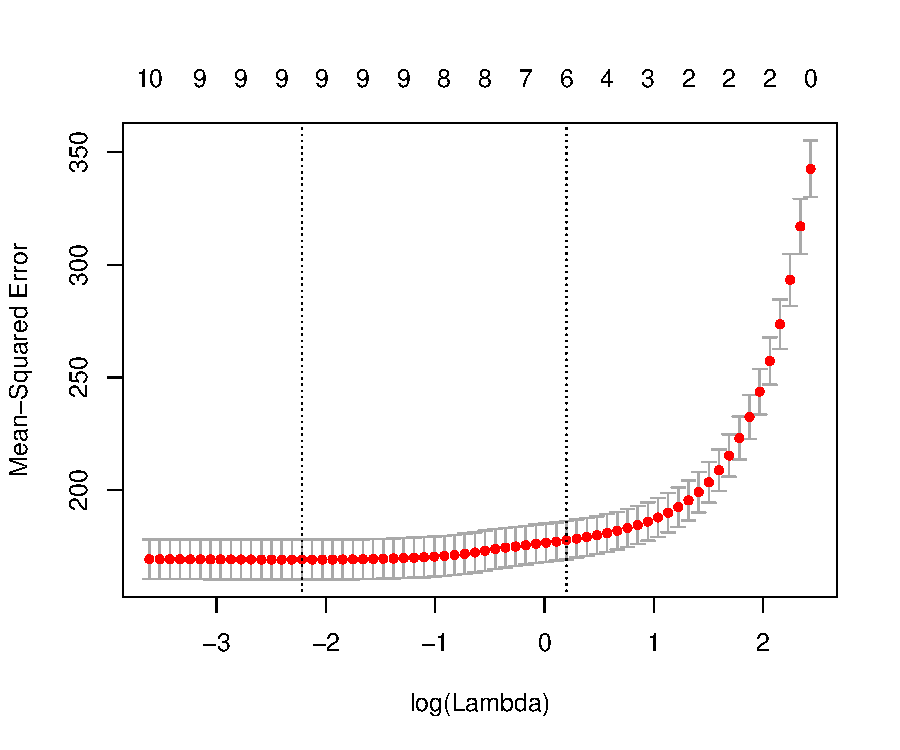
\includegraphics{Midterm_11_01_2016_Answers_files/figure-latex/unnamed-chunk-32-1} \end{flushleft}

\begin{Shaded}
\begin{Highlighting}[]
\CommentTok{# plot(fit.lasso.cv$lambda, fit.lasso.cv$cvm, xlab = expression(lambda),}
\CommentTok{# ylab='mean cv errors')}

\CommentTok{# OR}
\KeywordTok{set.seed}\NormalTok{(}\DecValTok{12}\NormalTok{)}
\NormalTok{fit_lasso <-}\StringTok{ }\KeywordTok{cv.glmnet}\NormalTok{(x_col, y_col, }\DataTypeTok{family =} \StringTok{"gaussian"}\NormalTok{, }\DataTypeTok{alpha =} \DecValTok{1}\NormalTok{)}
\KeywordTok{plot}\NormalTok{(fit_lasso, }\DataTypeTok{main =} \StringTok{"CMV vs Lambda in LASSO"}\NormalTok{)}
\end{Highlighting}
\end{Shaded}

\begin{flushleft}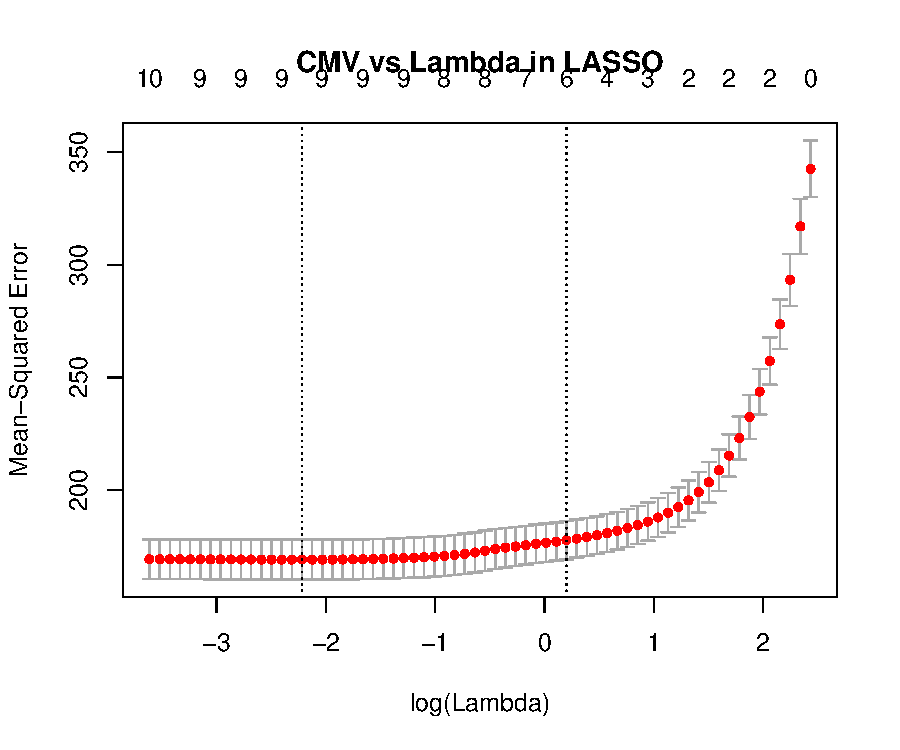
\includegraphics{Midterm_11_01_2016_Answers_files/figure-latex/unnamed-chunk-32-2} \end{flushleft}

\textbf{b)} What is the \texttt{lambda.1se} value? Under the
\texttt{lambda.1se} criterion, list the non-zero variables returned?

lambda 1se:

\begin{Shaded}
\begin{Highlighting}[]
\NormalTok{fit.lasso.cv}\OperatorTok{$}\NormalTok{lambda.1se}
\end{Highlighting}
\end{Shaded}

\begin{verbatim}
## [1] 1.222679
\end{verbatim}

\begin{Shaded}
\begin{Highlighting}[]
\CommentTok{# fit_lasso$lambda.1se}
\end{Highlighting}
\end{Shaded}

And we have the following variables in the model: Non-zero variables
are:

\begin{Shaded}
\begin{Highlighting}[]
\CommentTok{# <<<<<<<< COEFFICIENTS FROM LASSO, WITH 10 FOLD CROSS VALIDATION USING}
\CommentTok{# LAMBDA.1SE >>>>>>>> can choose any value between lambda.min and lambda.1se}
\NormalTok{coef_1se <-}\StringTok{ }\KeywordTok{coef}\NormalTok{(fit.lasso.cv, }\DataTypeTok{s =} \StringTok{"lambda.1se"}\NormalTok{)}
\NormalTok{nzcoef <-}\StringTok{ }\KeywordTok{rownames}\NormalTok{(coef_1se)[}\KeywordTok{which}\NormalTok{((coef_1se) }\OperatorTok{!=}\StringTok{ }\DecValTok{0}\NormalTok{)]}
\NormalTok{nzcoef}
\end{Highlighting}
\end{Shaded}

\begin{verbatim}
## [1] "(Intercept)"  "Schooltype2"  "All.test.std" "Acc.Rate"    
## [5] "Pct.Yield"    "In.Tuition"   "Room.board"
\end{verbatim}

\begin{Shaded}
\begin{Highlighting}[]
\NormalTok{lm.input <-}\StringTok{ }\KeywordTok{as.formula}\NormalTok{(}\KeywordTok{paste}\NormalTok{(}\StringTok{"Grad.rate"}\NormalTok{, }\StringTok{"~"}\NormalTok{, }\KeywordTok{paste}\NormalTok{(nzcoef[}\OperatorTok{-}\DecValTok{1}\NormalTok{], }\DataTypeTok{collapse =} \StringTok{"+"}\NormalTok{)))}
\NormalTok{lm.input}
\end{Highlighting}
\end{Shaded}

\begin{verbatim}
## Grad.rate ~ Schooltype2 + All.test.std + Acc.Rate + Pct.Yield + 
##     In.Tuition + Room.board
\end{verbatim}

\begin{Shaded}
\begin{Highlighting}[]
\CommentTok{# OR coefs_1se = coef(fit_lasso, s='lambda.1se')}
\CommentTok{# rownames(coefs_1se)[which((coefs_1se) != 0)]}
\end{Highlighting}
\end{Shaded}

Grad.rate \textasciitilde{} Schooltype2 + All.test.std + Acc.Rate +
Pct.Yield + In.Tuition + Room.board

\textbf{c)} \texttt{fit5}: Run OLS with all the variables returned from
part b), \textbf{and with State also included in the model}. Are all the
variables included here significant at the .01 level? If not, perform
backward elimination (manually) until all the p-values for the remaining
variables are less than .01. Show your model building process and report
the final LS equations. \emph{Note: for this problem, force State into
the final model, i.e., do not remove State.}

\begin{Shaded}
\begin{Highlighting}[]
\NormalTok{input5 <-}\StringTok{ }\NormalTok{Grad.rate }\OperatorTok{~}\StringTok{ }\NormalTok{Schooltype }\OperatorTok{+}\StringTok{ }\NormalTok{All.test.std }\OperatorTok{+}\StringTok{ }\NormalTok{Acc.Rate }\OperatorTok{+}\StringTok{ }\NormalTok{Pct.Yield }\OperatorTok{+}\StringTok{ }\NormalTok{In.Tuition }\OperatorTok{+}\StringTok{ }
\StringTok{    }\NormalTok{Room.board }\OperatorTok{+}\StringTok{ }\NormalTok{State}
\NormalTok{fit5 <-}\StringTok{ }\KeywordTok{lm}\NormalTok{(input5, }\DataTypeTok{data =}\NormalTok{ college_data)}
\KeywordTok{summary}\NormalTok{(fit5)}
\end{Highlighting}
\end{Shaded}

\begin{verbatim}
## 
## Call:
## lm(formula = input5, data = college_data)
## 
## Residuals:
##     Min      1Q  Median      3Q     Max 
## -40.755  -7.513  -0.266   6.890  45.168 
## 
## Coefficients:
##                Estimate Std. Error t value Pr(>|t|)    
## (Intercept)   1.221e+01  1.276e+01   0.957 0.338966    
## Schooltype2   9.703e+00  1.676e+00   5.788 9.56e-09 ***
## All.test.std  9.233e+00  5.826e-01  15.846  < 2e-16 ***
## Acc.Rate     -4.687e-02  3.152e-02  -1.487 0.137312    
## Pct.Yield    -3.992e-02  3.262e-02  -1.224 0.221323    
## In.Tuition   -9.898e-06  1.906e-04  -0.052 0.958587    
## Room.board    6.808e-04  5.885e-04   1.157 0.247607    
## StateAL       3.838e+01  1.259e+01   3.048 0.002368 ** 
## StateAR       3.743e+01  1.302e+01   2.875 0.004123 ** 
## StateAZ       4.355e+01  1.370e+01   3.180 0.001519 ** 
## StateCA       4.256e+01  1.237e+01   3.440 0.000606 ***
## StateCO       4.046e+01  1.276e+01   3.171 0.001564 ** 
## StateCT       5.324e+01  1.265e+01   4.209 2.80e-05 ***
## StateDC       4.814e+01  1.326e+01   3.630 0.000298 ***
## StateDE       5.084e+01  1.412e+01   3.600 0.000334 ***
## StateFL       4.155e+01  1.249e+01   3.326 0.000912 ***
## StateGA       4.007e+01  1.243e+01   3.223 0.001308 ** 
## StateHI       3.836e+01  1.502e+01   2.554 0.010799 *  
## StateIA       4.560e+01  1.251e+01   3.645 0.000281 ***
## StateID       3.357e+01  1.326e+01   2.532 0.011505 *  
## StateIL       4.692e+01  1.239e+01   3.787 0.000162 ***
## StateIN       4.833e+01  1.244e+01   3.885 0.000109 ***
## StateKS       3.900e+01  1.265e+01   3.083 0.002104 ** 
## StateKY       4.581e+01  1.265e+01   3.623 0.000307 ***
## StateLA       3.581e+01  1.266e+01   2.828 0.004779 ** 
## StateMA       5.236e+01  1.240e+01   4.223 2.64e-05 ***
## StateMD       4.337e+01  1.254e+01   3.458 0.000568 ***
## StateME       5.324e+01  1.281e+01   4.157 3.50e-05 ***
## StateMI       4.298e+01  1.249e+01   3.442 0.000602 ***
## StateMN       4.866e+01  1.259e+01   3.866 0.000118 ***
## StateMO       4.181e+01  1.250e+01   3.346 0.000852 ***
## StateMS       4.407e+01  1.287e+01   3.426 0.000638 ***
## StateMT       4.522e+01  1.313e+01   3.444 0.000598 ***
## StateNC       4.568e+01  1.238e+01   3.691 0.000236 ***
## StateND       4.024e+01  1.329e+01   3.028 0.002524 ** 
## StateNE       4.866e+01  1.294e+01   3.761 0.000179 ***
## StateNH       5.489e+01  1.280e+01   4.289 1.97e-05 ***
## StateNJ       4.397e+01  1.251e+01   3.516 0.000458 ***
## StateNM       3.393e+01  1.300e+01   2.610 0.009191 ** 
## StateNV       3.364e+01  1.501e+01   2.241 0.025266 *  
## StateNY       4.609e+01  1.233e+01   3.737 0.000197 ***
## StateOH       5.115e+01  1.241e+01   4.123 4.05e-05 ***
## StateOK       3.178e+01  1.274e+01   2.495 0.012775 *  
## StateOR       3.649e+01  1.272e+01   2.868 0.004214 ** 
## StatePA       5.492e+01  1.233e+01   4.453 9.42e-06 ***
## StateRI       5.709e+01  1.303e+01   4.381 1.31e-05 ***
## StateSC       5.301e+01  1.256e+01   4.222 2.65e-05 ***
## StateSD       4.706e+01  1.327e+01   3.545 0.000411 ***
## StateTN       3.892e+01  1.249e+01   3.117 0.001881 ** 
## StateTX       3.818e+01  1.238e+01   3.084 0.002097 ** 
## StateUT       2.986e+01  1.505e+01   1.984 0.047501 *  
## StateVA       4.944e+01  1.242e+01   3.981 7.37e-05 ***
## StateVT       5.711e+01  1.278e+01   4.468 8.83e-06 ***
## StateWA       4.849e+01  1.268e+01   3.823 0.000140 ***
## StateWI       4.684e+01  1.250e+01   3.746 0.000190 ***
## StateWV       5.190e+01  1.264e+01   4.105 4.37e-05 ***
## StateWY       3.423e+01  1.736e+01   1.972 0.048840 *  
## ---
## Signif. codes:  0 '***' 0.001 '**' 0.01 '*' 0.05 '.' 0.1 ' ' 1
## 
## Residual standard error: 12.23 on 985 degrees of freedom
## Multiple R-squared:  0.5886, Adjusted R-squared:  0.5652 
## F-statistic: 25.16 on 56 and 985 DF,  p-value: < 2.2e-16
\end{verbatim}

\begin{Shaded}
\begin{Highlighting}[]
\KeywordTok{Anova}\NormalTok{(fit5)}
\end{Highlighting}
\end{Shaded}

\begin{verbatim}
## Anova Table (Type II tests)
## 
## Response: Grad.rate
##              Sum Sq  Df  F value    Pr(>F)    
## Schooltype     5009   1  33.5018 9.564e-09 ***
## All.test.std  37548   1 251.1083 < 2.2e-16 ***
## Acc.Rate        331   1   2.2114    0.1373    
## Pct.Yield       224   1   1.4977    0.2213    
## In.Tuition        0   1   0.0027    0.9586    
## Room.board      200   1   1.3383    0.2476    
## State         30514  50   4.0813 < 2.2e-16 ***
## Residuals    147285 985                       
## ---
## Signif. codes:  0 '***' 0.001 '**' 0.01 '*' 0.05 '.' 0.1 ' ' 1
\end{verbatim}

kicking out \texttt{In.Tuition} because it has the smallest F-value
(0.0027) and largest P value(0.9586)

\begin{Shaded}
\begin{Highlighting}[]
\NormalTok{input5.}\DecValTok{1}\NormalTok{ <-}\StringTok{ }\NormalTok{Grad.rate }\OperatorTok{~}\StringTok{ }\NormalTok{Schooltype }\OperatorTok{+}\StringTok{ }\NormalTok{All.test.std }\OperatorTok{+}\StringTok{ }\NormalTok{Acc.Rate }\OperatorTok{+}\StringTok{ }\NormalTok{Pct.Yield }\OperatorTok{+}\StringTok{ }\NormalTok{Room.board }\OperatorTok{+}\StringTok{ }
\StringTok{    }\NormalTok{State}
\NormalTok{fit5.}\DecValTok{1}\NormalTok{ <-}\StringTok{ }\KeywordTok{lm}\NormalTok{(input5.}\DecValTok{1}\NormalTok{, }\DataTypeTok{data =}\NormalTok{ college_data)}
\CommentTok{# summary(fit5.1)}
\KeywordTok{Anova}\NormalTok{(fit5.}\DecValTok{1}\NormalTok{)}
\end{Highlighting}
\end{Shaded}

\begin{verbatim}
## Anova Table (Type II tests)
## 
## Response: Grad.rate
##              Sum Sq  Df  F value Pr(>F)    
## Schooltype    15623   1 104.5910 <2e-16 ***
## All.test.std  50991   1 341.3624 <2e-16 ***
## Acc.Rate        330   1   2.2123 0.1372    
## Pct.Yield       225   1   1.5086 0.2197    
## Room.board      215   1   1.4387 0.2306    
## State         32255  50   4.3186 <2e-16 ***
## Residuals    147285 986                    
## ---
## Signif. codes:  0 '***' 0.001 '**' 0.01 '*' 0.05 '.' 0.1 ' ' 1
\end{verbatim}

Now kicking out \texttt{Room.board}.

\begin{Shaded}
\begin{Highlighting}[]
\NormalTok{input5.}\DecValTok{2}\NormalTok{ <-}\StringTok{ }\NormalTok{Grad.rate }\OperatorTok{~}\StringTok{ }\NormalTok{Schooltype }\OperatorTok{+}\StringTok{ }\NormalTok{All.test.std }\OperatorTok{+}\StringTok{ }\NormalTok{Acc.Rate }\OperatorTok{+}\StringTok{ }\NormalTok{Pct.Yield }\OperatorTok{+}\StringTok{ }\NormalTok{State}
\NormalTok{fit5.}\DecValTok{2}\NormalTok{ <-}\StringTok{ }\KeywordTok{lm}\NormalTok{(input5.}\DecValTok{2}\NormalTok{, }\DataTypeTok{data =}\NormalTok{ college_data)}
\CommentTok{# summary(fit5.2)}
\KeywordTok{Anova}\NormalTok{(fit5.}\DecValTok{2}\NormalTok{)}
\end{Highlighting}
\end{Shaded}

\begin{verbatim}
## Anova Table (Type II tests)
## 
## Response: Grad.rate
##              Sum Sq  Df  F value Pr(>F)    
## Schooltype    19206   1 128.5169 <2e-16 ***
## All.test.std  62060   1 415.2794 <2e-16 ***
## Acc.Rate        345   1   2.3108 0.1288    
## Pct.Yield       301   1   2.0161 0.1560    
## State         34830  50   4.6614 <2e-16 ***
## Residuals    147500 987                    
## ---
## Signif. codes:  0 '***' 0.001 '**' 0.01 '*' 0.05 '.' 0.1 ' ' 1
\end{verbatim}

Now kicking out \texttt{Pct.Yield}.

\begin{Shaded}
\begin{Highlighting}[]
\NormalTok{input5.}\DecValTok{3}\NormalTok{ <-}\StringTok{ }\NormalTok{Grad.rate }\OperatorTok{~}\StringTok{ }\NormalTok{Schooltype }\OperatorTok{+}\StringTok{ }\NormalTok{All.test.std }\OperatorTok{+}\StringTok{ }\NormalTok{Acc.Rate }\OperatorTok{+}\StringTok{ }\NormalTok{State}
\NormalTok{fit5.}\DecValTok{3}\NormalTok{ <-}\StringTok{ }\KeywordTok{lm}\NormalTok{(input5.}\DecValTok{3}\NormalTok{, }\DataTypeTok{data =}\NormalTok{ college_data)}
\CommentTok{# summary(fit5.3)}
\KeywordTok{Anova}\NormalTok{(fit5.}\DecValTok{3}\NormalTok{)}
\end{Highlighting}
\end{Shaded}

\begin{verbatim}
## Anova Table (Type II tests)
## 
## Response: Grad.rate
##              Sum Sq  Df  F value Pr(>F)    
## Schooltype    20448   1 136.6892 <2e-16 ***
## All.test.std  67537   1 451.4632 <2e-16 ***
## Acc.Rate        278   1   1.8583 0.1731    
## State         40152  50   5.3680 <2e-16 ***
## Residuals    147801 988                    
## ---
## Signif. codes:  0 '***' 0.001 '**' 0.01 '*' 0.05 '.' 0.1 ' ' 1
\end{verbatim}

Kicking out last var-- \texttt{Acc.Rate}.

\begin{Shaded}
\begin{Highlighting}[]
\NormalTok{input5.}\DecValTok{4}\NormalTok{ <-}\StringTok{ }\NormalTok{Grad.rate }\OperatorTok{~}\StringTok{ }\NormalTok{Schooltype }\OperatorTok{+}\StringTok{ }\NormalTok{All.test.std }\OperatorTok{+}\StringTok{ }\NormalTok{State}
\NormalTok{fit5.}\DecValTok{4}\NormalTok{ <-}\StringTok{ }\KeywordTok{lm}\NormalTok{(input5.}\DecValTok{4}\NormalTok{, }\DataTypeTok{data =}\NormalTok{ college_data)}
\CommentTok{# summary(fit5.4)}
\KeywordTok{Anova}\NormalTok{(fit5.}\DecValTok{4}\NormalTok{)}
\end{Highlighting}
\end{Shaded}

\begin{verbatim}
## Anova Table (Type II tests)
## 
## Response: Grad.rate
##              Sum Sq  Df  F value    Pr(>F)    
## Schooltype    20239   1 135.1712 < 2.2e-16 ***
## All.test.std  88427   1 590.5889 < 2.2e-16 ***
## State         42005  50   5.6109 < 2.2e-16 ***
## Residuals    148079 989                       
## ---
## Signif. codes:  0 '***' 0.001 '**' 0.01 '*' 0.05 '.' 0.1 ' ' 1
\end{verbatim}

\textbf{Better way to do it}

\begin{Shaded}
\begin{Highlighting}[]
\NormalTok{fit5 =}\StringTok{ }\KeywordTok{lm}\NormalTok{(Grad.rate }\OperatorTok{~}\StringTok{ }\NormalTok{State }\OperatorTok{+}\StringTok{ }\NormalTok{Schooltype }\OperatorTok{+}\StringTok{ }\NormalTok{All.test.std }\OperatorTok{+}\StringTok{ }\NormalTok{Acc.Rate }\OperatorTok{+}\StringTok{ }\NormalTok{Pct.Yield }\OperatorTok{+}\StringTok{ }
\StringTok{    }\NormalTok{In.Tuition }\OperatorTok{+}\StringTok{ }\NormalTok{Room.board, }\DataTypeTok{data =}\NormalTok{ college_data)}
\end{Highlighting}
\end{Shaded}

\begin{Shaded}
\begin{Highlighting}[]
\KeywordTok{Anova}\NormalTok{(fit5)}

\CommentTok{# remove In.Tuition}
\NormalTok{fit5_}\DecValTok{1}\NormalTok{ =}\StringTok{ }\KeywordTok{update}\NormalTok{(fit5, . }\OperatorTok{~}\StringTok{ }\NormalTok{. }\OperatorTok{-}\StringTok{ }\NormalTok{In.Tuition)}
\KeywordTok{Anova}\NormalTok{(fit5_}\DecValTok{1}\NormalTok{)}

\CommentTok{# remove Room.Board}
\NormalTok{fit5_}\DecValTok{2}\NormalTok{ =}\StringTok{ }\KeywordTok{update}\NormalTok{(fit5_}\DecValTok{1}\NormalTok{, . }\OperatorTok{~}\StringTok{ }\NormalTok{. }\OperatorTok{-}\StringTok{ }\NormalTok{Room.board)}
\KeywordTok{Anova}\NormalTok{(fit5_}\DecValTok{2}\NormalTok{)}

\CommentTok{# remove Pct.Yield}
\NormalTok{fit5_}\DecValTok{3}\NormalTok{ =}\StringTok{ }\KeywordTok{update}\NormalTok{(fit5_}\DecValTok{2}\NormalTok{, . }\OperatorTok{~}\StringTok{ }\NormalTok{. }\OperatorTok{-}\StringTok{ }\NormalTok{Pct.Yield)}
\KeywordTok{Anova}\NormalTok{(fit5_}\DecValTok{3}\NormalTok{)}

\CommentTok{# remove Acc.Rate}
\NormalTok{fit5_}\DecValTok{4}\NormalTok{ =}\StringTok{ }\KeywordTok{update}\NormalTok{(fit5_}\DecValTok{3}\NormalTok{, . }\OperatorTok{~}\StringTok{ }\NormalTok{. }\OperatorTok{-}\StringTok{ }\NormalTok{Acc.Rate)}
\KeywordTok{Anova}\NormalTok{(fit5_}\DecValTok{4}\NormalTok{)}
\end{Highlighting}
\end{Shaded}

We see that our final model is \texttt{Grad.rate} \textasciitilde{}
\texttt{State\ +\ Schooltype\ +\ All.test.std} :)

\section{Question 6: Graduation
Evaluation}\label{question-6-graduation-evaluation}

Independent of Question 5. Assume that this we've decided to use
\texttt{fit6} as our final model.

\texttt{fit6}: \texttt{Grad.rate} \textasciitilde{}
\texttt{State\ +\ Schooltype\ +\ All.test.std}

\begin{Shaded}
\begin{Highlighting}[]
\NormalTok{fit6 <-}\StringTok{ }\KeywordTok{lm}\NormalTok{(Grad.rate }\OperatorTok{~}\StringTok{ }\NormalTok{State }\OperatorTok{+}\StringTok{ }\NormalTok{Schooltype }\OperatorTok{+}\StringTok{ }\NormalTok{All.test.std, }\DataTypeTok{data =}\NormalTok{ college_data)}
\KeywordTok{Anova}\NormalTok{(fit6)}
\end{Highlighting}
\end{Shaded}

\begin{verbatim}
## Anova Table (Type II tests)
## 
## Response: Grad.rate
##              Sum Sq  Df  F value    Pr(>F)    
## State         42005  50   5.6109 < 2.2e-16 ***
## Schooltype    20239   1 135.1712 < 2.2e-16 ***
## All.test.std  88427   1 590.5889 < 2.2e-16 ***
## Residuals    148079 989                       
## ---
## Signif. codes:  0 '***' 0.001 '**' 0.01 '*' 0.05 '.' 0.1 ' ' 1
\end{verbatim}

\textbf{a)} Are all three variables significant at .01 level? Yep

\begin{Shaded}
\begin{Highlighting}[]
\NormalTok{car}\OperatorTok{::}\KeywordTok{Anova}\NormalTok{(fit6)}
\end{Highlighting}
\end{Shaded}

\begin{verbatim}
## Anova Table (Type II tests)
## 
## Response: Grad.rate
##              Sum Sq  Df  F value    Pr(>F)    
## State         42005  50   5.6109 < 2.2e-16 ***
## Schooltype    20239   1 135.1712 < 2.2e-16 ***
## All.test.std  88427   1 590.5889 < 2.2e-16 ***
## Residuals    148079 989                       
## ---
## Signif. codes:  0 '***' 0.001 '**' 0.01 '*' 0.05 '.' 0.1 ' ' 1
\end{verbatim}

\textbf{b)} Provide the residual plot.

\begin{Shaded}
\begin{Highlighting}[]
\CommentTok{# <<<<<<<<<< RESIDUAL PLOT -- LINEARITY & HOMOSCEDASTICITY >>>>>>>>>}
\KeywordTok{plot}\NormalTok{(fit6}\OperatorTok{$}\NormalTok{fitted.values, fit6}\OperatorTok{$}\NormalTok{residuals, }\DataTypeTok{pch =} \DecValTok{16}\NormalTok{, }\DataTypeTok{main =} \StringTok{"residual plot"}\NormalTok{)}
\KeywordTok{abline}\NormalTok{(}\DataTypeTok{h =} \DecValTok{0}\NormalTok{, }\DataTypeTok{lwd =} \DecValTok{4}\NormalTok{, }\DataTypeTok{col =} \StringTok{"red"}\NormalTok{)}
\end{Highlighting}
\end{Shaded}

\begin{flushleft}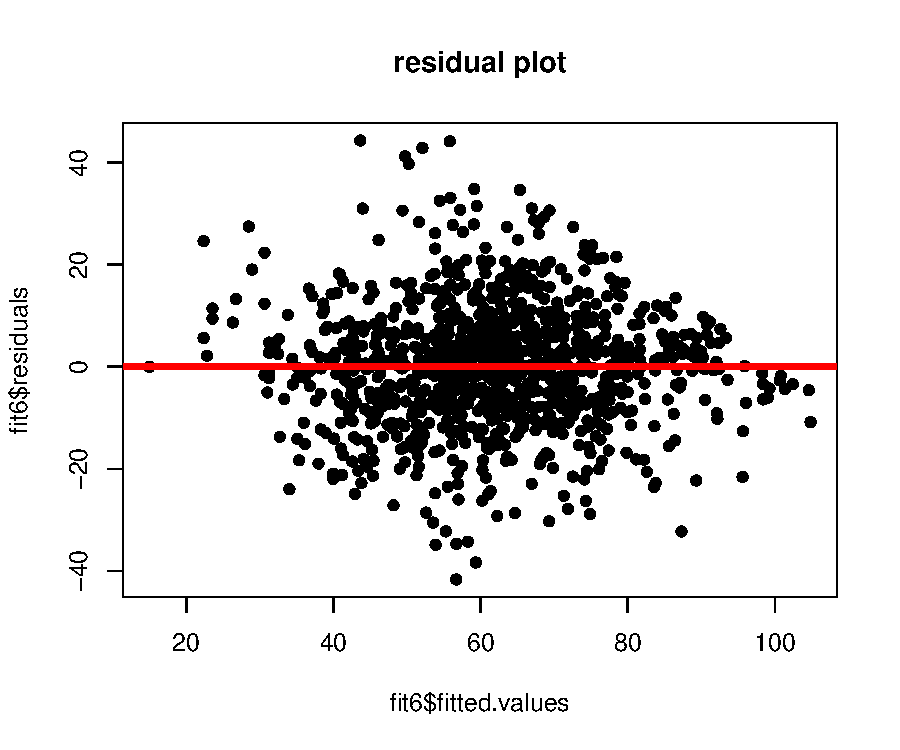
\includegraphics{Midterm_11_01_2016_Answers_files/figure-latex/unnamed-chunk-44-1} \end{flushleft}

\begin{Shaded}
\begin{Highlighting}[]
\KeywordTok{plot}\NormalTok{(fit6}\OperatorTok{$}\NormalTok{fitted, fit6}\OperatorTok{$}\NormalTok{residuals)}
\end{Highlighting}
\end{Shaded}

\begin{flushleft}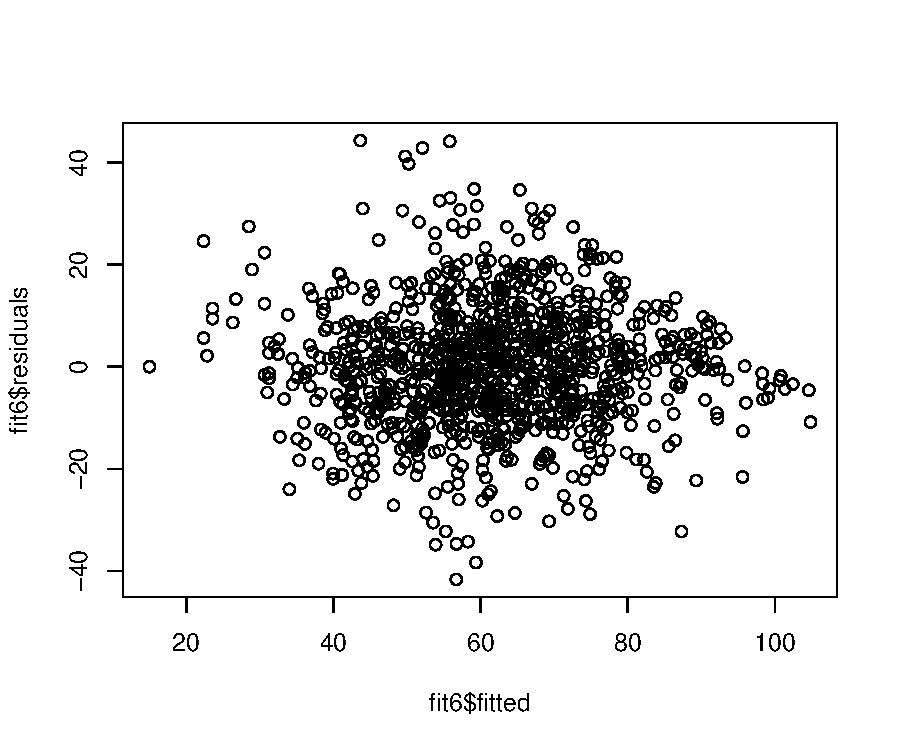
\includegraphics{Midterm_11_01_2016_Answers_files/figure-latex/unnamed-chunk-45-1} \end{flushleft}

\textbf{c)} Provide the qqnorm plot of the residuals.

\begin{Shaded}
\begin{Highlighting}[]
\CommentTok{# <<<<<<<< QQNORM PLOT FOR NORMALITY >>>>>>>>>}
\KeywordTok{qqnorm}\NormalTok{(fit6}\OperatorTok{$}\NormalTok{residuals)}
\KeywordTok{qqline}\NormalTok{(fit6}\OperatorTok{$}\NormalTok{residuals, }\DataTypeTok{lwd =} \DecValTok{4}\NormalTok{, }\DataTypeTok{col =} \StringTok{"blue"}\NormalTok{)}
\end{Highlighting}
\end{Shaded}

\begin{flushleft}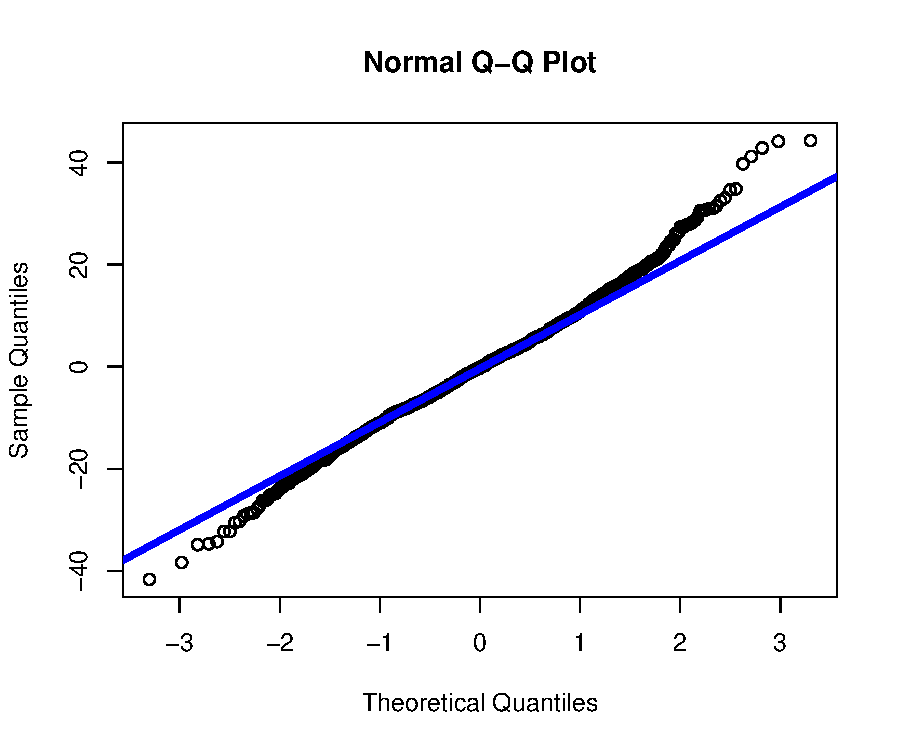
\includegraphics{Midterm_11_01_2016_Answers_files/figure-latex/unnamed-chunk-46-1} \end{flushleft}

\begin{Shaded}
\begin{Highlighting}[]
\KeywordTok{qqnorm}\NormalTok{(fit6}\OperatorTok{$}\NormalTok{residuals)}
\KeywordTok{qqline}\NormalTok{(fit6}\OperatorTok{$}\NormalTok{residuals)}
\end{Highlighting}
\end{Shaded}

\begin{flushleft}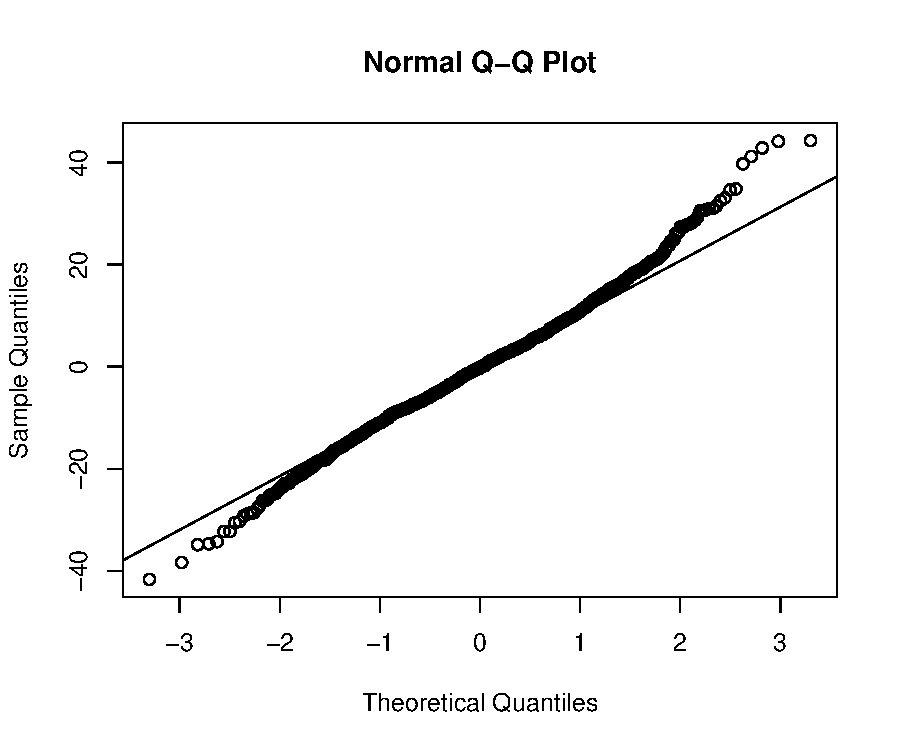
\includegraphics{Midterm_11_01_2016_Answers_files/figure-latex/unnamed-chunk-47-1} \end{flushleft}

\textbf{d)} Do the model meet all the linear model assumptions?

Yeah

\textbf{e)} Finally, using \texttt{fit6}, provide a 95\% prediction
interval for Penn's graduation rate. Based on Penn's actual graduation
rate, how do you think of the performance of our prediction?

\begin{Shaded}
\begin{Highlighting}[]
\CommentTok{# penn_loc <- which(college_data$Name == 'University of Pennsylvania') #}
\CommentTok{# identify Penn Penn <- college_data[penn_loc, ] Penn `State + Schooltype +}
\CommentTok{# All.test.std` pred <- data.frame(State = 'Pennsylvania', Schooltype = '2',}
\CommentTok{# All.test.std = .5765) # margin calculated from dem - republican vote pred}
\KeywordTok{predict}\NormalTok{(fit6, Penn, }\DataTypeTok{interval =} \StringTok{"prediction"}\NormalTok{, }\DataTypeTok{se =} \OtherTok{FALSE}\NormalTok{)}
\end{Highlighting}
\end{Shaded}

\begin{verbatim}
##          fit      lwr      upr
## 820 99.04858 74.81411 123.2831
\end{verbatim}

\begin{Shaded}
\begin{Highlighting}[]
\CommentTok{# OR predict(fit6, newdata = filter(college_data, Name == 'University of}
\CommentTok{# Pennsylvania'), interval = 'prediction', level = 0.95)}
\end{Highlighting}
\end{Shaded}

The prediction interval is 74.81 to 123\%, which I guess isn't great
because our upper bound is over 100\%, but is acceptable. Our fit is at
99\%, and Penn's real graduation rate is 93, indicating that this school
is underperforming our model, but at least taught us enough statistics
to get a prediction interval containing the true rate.

\section{Question 7: Freedom of the
Press}\label{question-7-freedom-of-the-press}

Newsweek did a great job of collecting graduate data, but some schools
are unhappy with their exact graduation figures being reported. They
lobbied Newsweek's publisher to report only whether a school's
graduation rate is either High (\texttt{Grad.rate\ \textgreater{}=\ 70})
or Low (\texttt{Grad.rate\ \textless{}\ 70}); the ``journalists''
acquiesced to their corporate overlords. From now on, the only
graduation rate data available to you is in that high/low form.

\textbf{a)} Create a new categorical variable \texttt{Grad.rate.2} in
\texttt{college\_data} that fits the new specification. What proportion
of the schools are categorized as ``High Graduation'', that is,
\texttt{Grad.rate.2\ ==\ "1"}?

\begin{Shaded}
\begin{Highlighting}[]
\CommentTok{# limit <- 70 #Grad.rate2 <- factor(ifelse(college_data$Grad.rate >= limit,}
\CommentTok{# '1', '0')) Grad.rate.2 <- ifelse(college_data$Grad.rate >= limit, '1',}
\CommentTok{# '0') Grad.rate.2 summary(Grad.rate.2)}

\NormalTok{college_data }\OperatorTok\StringTok{ }\KeywordTok{mutate}\NormalTok{(}\DataTypeTok{Grad.rate.2 =} \KeywordTok{as.factor}\NormalTok{(}\KeywordTok{as.numeric}\NormalTok{(Grad.rate }\OperatorTok{>=}\StringTok{ }\DecValTok{70}\NormalTok{)))}
\KeywordTok{table}\NormalTok{(college_data}\OperatorTok{$}\NormalTok{Grad.rate.}\DecValTok{2}\NormalTok{)}\OperatorTok{/}\KeywordTok{nrow}\NormalTok{(college_data)}
\end{Highlighting}
\end{Shaded}

\begin{verbatim}
## 
##        0        1 
## 0.659309 0.340691
\end{verbatim}

34.06\% of colleges have ``high'' graduation rates.

\textbf{b)} How well can we predict \texttt{Grad.rate.2}, with only
three variables: \texttt{State}, \texttt{Schooltype} and
\texttt{All.test.std}. Run a logistic regression of \texttt{Grad.rate.2}
vs. \texttt{State}, \texttt{Schooltype} and \texttt{All.test.std}. Is
every variable significant at .01 level, whilst controlling the other
two variables?

\begin{Shaded}
\begin{Highlighting}[]
\CommentTok{# lm.categor <- lm(Grad.rate.2 ~ State + Schooltype + All.test.std, data =}
\CommentTok{# college_data) summary(lm.categor) Anova(lm.categor) NOT WORKING}
\end{Highlighting}
\end{Shaded}

Each variable is significant at 0.01, while controlling for the other
variables.

\begin{Shaded}
\begin{Highlighting}[]
\NormalTok{fit7 <-}\StringTok{ }\KeywordTok{glm}\NormalTok{(Grad.rate.}\DecValTok{2} \OperatorTok{~}\StringTok{ }\NormalTok{State }\OperatorTok{+}\StringTok{ }\NormalTok{Schooltype }\OperatorTok{+}\StringTok{ }\NormalTok{All.test.std, }\DataTypeTok{data =}\NormalTok{ college_data, }
    \DataTypeTok{family =} \StringTok{"binomial"}\NormalTok{)}
\NormalTok{car}\OperatorTok{::}\KeywordTok{Anova}\NormalTok{(fit7)}
\end{Highlighting}
\end{Shaded}

\begin{verbatim}
## Analysis of Deviance Table (Type II tests)
## 
## Response: Grad.rate.2
##              LR Chisq Df Pr(>Chisq)    
## State         141.269 50  1.212e-10 ***
## Schooltype     71.555  1  < 2.2e-16 ***
## All.test.std  200.264  1  < 2.2e-16 ***
## ---
## Signif. codes:  0 '***' 0.001 '**' 0.01 '*' 0.05 '.' 0.1 ' ' 1
\end{verbatim}

\begin{Shaded}
\begin{Highlighting}[]
\KeywordTok{dim}\NormalTok{(college_data)}
\end{Highlighting}
\end{Shaded}

\begin{verbatim}
## [1] 1042   14
\end{verbatim}

\textbf{c)} Let us fix our classification threshold to 0.5, that is, we
will classify the school to be ``High Graduation'' if
\(\hat{P}\)\texttt{(Grad.rate.2\ ==\ "1")\ \textgreater{}\ 0.5} (the
estimated probability of being ``High Graduation'' is greater than 0.5).
Under this framework, what is the in-sample mis-classification error?
Show your work.

\begin{Shaded}
\begin{Highlighting}[]
\KeywordTok{library}\NormalTok{(caret)}
\end{Highlighting}
\end{Shaded}

\begin{verbatim}
## Loading required package: lattice
\end{verbatim}

\begin{Shaded}
\begin{Highlighting}[]
\CommentTok{# fit7 -- normal logistic regression fit7.1 -- logistic regression with .5}
\CommentTok{# threshold fit7.output1 -- categorized df with 10 randomly chosen entries}

\NormalTok{fit7.}\DecValTok{1}\NormalTok{ <-}\StringTok{ }\KeywordTok{ifelse}\NormalTok{(fit7}\OperatorTok{$}\NormalTok{fitted.values }\OperatorTok{>}\StringTok{ }\DecValTok{1}\OperatorTok{/}\DecValTok{2}\NormalTok{, }\StringTok{"1"}\NormalTok{, }\StringTok{"0"}\NormalTok{)}
\KeywordTok{set.seed}\NormalTok{(}\DecValTok{10}\NormalTok{)}
\NormalTok{fit7.output1 <-}\StringTok{ }\KeywordTok{data.frame}\NormalTok{(college_data}\OperatorTok{$}\NormalTok{Grad.rate.}\DecValTok{2}\NormalTok{, fit7.}\DecValTok{1}\NormalTok{, fit7}\OperatorTok{$}\NormalTok{fitted.values)[}\KeywordTok{sample}\NormalTok{(}\DecValTok{1042}\NormalTok{, }
    \DecValTok{10}\NormalTok{), ]}
\KeywordTok{names}\NormalTok{(fit7.output1) <-}\StringTok{ }\KeywordTok{c}\NormalTok{(}\StringTok{"Y"}\NormalTok{, }\StringTok{"Predicted Y"}\NormalTok{, }\StringTok{"Prob"}\NormalTok{)}
\NormalTok{fit7.output1}
\end{Highlighting}
\end{Shaded}

\begin{verbatim}
##      Y Predicted Y       Prob
## 529  0           0 0.01041002
## 320  0           0 0.23185214
## 444  1           1 0.60159310
## 721  0           0 0.07095961
## 89   1           0 0.41700150
## 234  1           1 0.82189008
## 285  0           0 0.24971173
## 282  1           0 0.13224288
## 637  0           1 0.56410735
## 1040 0           0 0.38100593
\end{verbatim}

\begin{Shaded}
\begin{Highlighting}[]
\CommentTok{# confusion matrix}
\NormalTok{cm.fit7.}\DecValTok{5}\NormalTok{ <-}\StringTok{ }\KeywordTok{table}\NormalTok{(fit7.}\DecValTok{1}\NormalTok{, college_data}\OperatorTok{$}\NormalTok{Grad.rate.}\DecValTok{2}\NormalTok{)}
\NormalTok{cm.fit7.}\DecValTok{5}
\end{Highlighting}
\end{Shaded}

\begin{verbatim}
##       
## fit7.1   0   1
##      0 599 128
##      1  88 227
\end{verbatim}

\begin{Shaded}
\begin{Highlighting}[]
\CommentTok{# OR confusion matrix}
\KeywordTok{confusionMatrix}\NormalTok{(}\DataTypeTok{data =}\NormalTok{ fit7.}\DecValTok{1}\NormalTok{, }\DataTypeTok{reference =}\NormalTok{ college_data}\OperatorTok{$}\NormalTok{Grad.rate.}\DecValTok{2}\NormalTok{, }\DataTypeTok{positive =} \KeywordTok{levels}\NormalTok{(fit7.}\DecValTok{1}\NormalTok{)[}\DecValTok{2}\NormalTok{])}
\end{Highlighting}
\end{Shaded}

\begin{verbatim}
## Confusion Matrix and Statistics
## 
##           Reference
## Prediction   0   1
##          0 599 128
##          1  88 227
##                                           
##                Accuracy : 0.7927          
##                  95% CI : (0.7668, 0.8169)
##     No Information Rate : 0.6593          
##     P-Value [Acc > NIR] : < 2.2e-16       
##                                           
##                   Kappa : 0.5257          
##  Mcnemar's Test P-Value : 0.007963        
##                                           
##             Sensitivity : 0.8719          
##             Specificity : 0.6394          
##          Pos Pred Value : 0.8239          
##          Neg Pred Value : 0.7206          
##              Prevalence : 0.6593          
##          Detection Rate : 0.5749          
##    Detection Prevalence : 0.6977          
##       Balanced Accuracy : 0.7557          
##                                           
##        'Positive' Class : 0               
## 
\end{verbatim}

\begin{Shaded}
\begin{Highlighting}[]
\CommentTok{# MCE fit7.1 0 1 0 599 128 1 88 227 cm.fit7.5[1,2] #128 cm.fit7.5[2,1] #88}
\CommentTok{# length(fit7.1) #1042}
\NormalTok{error.training <-}\StringTok{ }\NormalTok{(cm.fit7.}\DecValTok{5}\NormalTok{[}\DecValTok{1}\NormalTok{, }\DecValTok{2}\NormalTok{] }\OperatorTok{+}\StringTok{ }\NormalTok{cm.fit7.}\DecValTok{5}\NormalTok{[}\DecValTok{2}\NormalTok{, }\DecValTok{1}\NormalTok{])}\OperatorTok{/}\KeywordTok{length}\NormalTok{(fit7.}\DecValTok{1}\NormalTok{)}
\NormalTok{error.training}
\end{Highlighting}
\end{Shaded}

\begin{verbatim}
## [1] 0.2072937
\end{verbatim}

\textbf{OR}

\begin{Shaded}
\begin{Highlighting}[]
\NormalTok{con_mat <-}\StringTok{ }\KeywordTok{table}\NormalTok{(fit7}\OperatorTok{$}\NormalTok{fitted.values }\OperatorTok{>}\StringTok{ }\FloatTok{0.5}\NormalTok{, college_data}\OperatorTok{$}\NormalTok{Grad.rate.}\DecValTok{2}\NormalTok{)}

\DecValTok{1} \OperatorTok{-}\StringTok{ }\KeywordTok{sum}\NormalTok{(}\KeywordTok{diag}\NormalTok{(con_mat))}\OperatorTok{/}\KeywordTok{nrow}\NormalTok{(college_data)}
\end{Highlighting}
\end{Shaded}

\begin{verbatim}
## [1] 0.2072937
\end{verbatim}

\begin{Shaded}
\begin{Highlighting}[]
\CommentTok{# sum of matrix diagonals is # of correctly predicted values 1 - correct =}
\CommentTok{# MCE}
\end{Highlighting}
\end{Shaded}

\vspace{.5in}

\subsection{END}\label{end}


\end{document}
